\documentclass[10pt]{article}

\usepackage{cmap}
\usepackage[T1]{fontenc}
\usepackage[utf8]{inputenc}
\usepackage{lmodern}
\usepackage[paperwidth=6.75in,paperheight=10in,top=0.68in,bottom=0.68in,left=0.68in,right=0.68in,headheight=13pt,headsep=16pt,footskip=24pt]{geometry}
\usepackage{amsmath}
\usepackage{array}
\usepackage{booktabs}
\usepackage{cite}
\usepackage{float}
\usepackage{graphicx}
\usepackage{longtable}
\usepackage{microtype}
\usepackage{caption}
\usepackage{fancyhdr}
\usepackage{titlesec}
\usepackage{tabularx}
\usepackage{url}
\usepackage{listings}
\usepackage[table]{xcolor}
\usepackage{tikz}
\usetikzlibrary{arrows.meta,fit,positioning}
\definecolor{ACMBlue}{RGB}{28,86,143}
\definecolor{ACMRule}{RGB}{72,72,72}
\definecolor{ACMTableHead}{RGB}{238,242,246}
\usepackage[colorlinks=true,linkcolor=ACMBlue,citecolor=ACMBlue,urlcolor=ACMBlue]{hyperref}
\linespread{1.02}
\setlength{\parindent}{1.15em}
\setlength{\parskip}{0pt}
\setlength{\emergencystretch}{2em}
\setlength{\tabcolsep}{4.5pt}
\setlength{\textfloatsep}{11pt plus 2pt minus 2pt}
\setlength{\intextsep}{9pt plus 2pt minus 2pt}

\titleformat{\section}{\large\bfseries}{\thesection}{0.65em}{}
\titleformat{\subsection}{\normalsize\bfseries}{\thesubsection}{0.65em}{}
\titleformat{\subsubsection}{\normalsize\bfseries}{\thesubsubsection}{0.65em}{}
\titlespacing*{\section}{0pt}{1.65em}{0.55em}
\titlespacing*{\subsection}{0pt}{1.25em}{0.4em}
\titlespacing*{\subsubsection}{0pt}{1em}{0.35em}

\captionsetup{font=small,labelfont=bf,labelsep=period,justification=centering,skip=5pt}
\captionsetup[table]{position=top}

\pagestyle{fancy}
\fancyhf{}
\fancyhead[L]{\footnotesize Trade-off-aware Evaluation of LLM-based Code Review}
\fancyhead[R]{\footnotesize Malverdi and Haghighi}
\fancyfoot[L]{\scriptsize Targeted Structured Review}
\fancyfoot[R]{\scriptsize\thepage}
\renewcommand{\headrulewidth}{0.35pt}
\renewcommand{\footrulewidth}{0.35pt}
\fancypagestyle{plain}{%
  \fancyhf{}%
  \fancyfoot[R]{\scriptsize\thepage}%
  \renewcommand{\headrulewidth}{0pt}%
  \renewcommand{\footrulewidth}{0.35pt}%
}

\lstset{
  basicstyle=\ttfamily\small,
  breaklines=true,
  columns=fullflexible,
  frame=single
}

\renewenvironment{abstract}{%
  \vspace{0.7em}\noindent\rule{\linewidth}{0.5pt}\par
  \vspace{0.55em}\noindent\textbf{ABSTRACT}\par\small\noindent
}{\par\normalsize\vspace{0.35em}}

\newcommand{\keywords}[1]{%
  \vspace{0.45em}
  \noindent\textbf{Additional Key Words and Phrases: }#1
}

\begin{document}
\thispagestyle{plain}
\begin{flushleft}
{\LARGE\bfseries Trade-off-aware Evaluation of LLM-based Code Review: A Structured Review of Comment Quality, Mitigation, and Evaluation Validity\par}
\vspace{1.25em}
{\large\bfseries MAHDI MALVERDI}, Shahid Beheshti University, Tehran, Iran\\
{\large\bfseries HASSAN HAGHIGHI}, Shahid Beheshti University, Tehran, Iran\\
\vspace{0.35em}
{\small \href{mailto:m.malverdi@mail.sbu.ac.ir}{m.malverdi@mail.sbu.ac.ir} \quad
\href{mailto:h_haghighi@sbu.ac.ir}{h\_haghighi@sbu.ac.ir}}
\end{flushleft}

% Source: drafts/paper/sections/00-abstract.md

\begin{abstract}
Large language models can produce fluent code review comments that are unsupported, irrelevant, difficult to act on, or costly to verify. Evaluating such feedback requires more than lexical similarity or acceptance because correctness, grounding, usefulness, and workflow value describe different properties. This targeted structured literature review synthesizes 121 full-text studies of automated code review and related evaluation methods. The evidence was organized through quality appraisal, evidence tiers, and thematic analysis. The review finds that failures can originate in the comment, the supplied context and data, the review workflow, or the evaluation procedure. It also finds that mitigation creates trade-offs: filtering, retrieval, verification, and rewriting may reduce one risk while losing useful feedback, narrowing review or issue coverage, increasing human escalation, or adding computational cost. These consequences are reported inconsistently across the corpus. Context can introduce noise or contradictory evidence, while LLM-as-a-Judge evaluation can be sensitive to prompts, ordering, model choice, and adversarial cues. Based on this synthesis, the paper proposes a failure taxonomy and a six-layer framework that links assessment to decisions to show, suppress, rewrite, or escalate feedback. The proposed taxonomy and framework still require independent empirical validation.
\end{abstract}
\keywords{LLM-based code review; automated code review; evaluation framework; problematic comments; context quality; LLM-as-a-Judge}



% Source: drafts/paper/sections/01-introduction.md

\section{Introduction}

A generated review comment can be inexpensive to produce but costly to handle. Once it appears in a pull request, a developer must decide whether to trust, verify, ignore, revise, or act on it. The comment therefore becomes part of a socio-technical workflow that supports not only defect detection but also maintainability, knowledge sharing, team awareness, and shared ownership \cite{p37_sadowski2018_google_mcr,p38_bacchelli2013_expectations_mcr,p39_bosu2015_useful_reviews,p51_davila2021_mcr_slr_taxonomy}.

LLM-based review systems now generate comments, suggest fixes, classify feedback, incorporate project context, and support security or static-analysis workflows \cite{p14_li2022_codereviewer,p19_nguyen2025_fine_grained_classification,p21_peng2025_icodereviewer,p22_jaoua2025_static_analyzers}. More recent systems distribute review across repository-level retrieval, tools, and agent trajectories \cite{p74_charoenwet2026_agentic_code_review_in_the_ter,p76_wang2026_swe_review_closing_the_loop_on,p85_zhang2026_reporeviewer_a_local_first_mul}. Evaluation has also moved toward richer rubrics, PR-level benchmarks, industrial telemetry, and human-centered studies \cite{p01_lu2025_deepcrceval,p03_tantithamthavorn2026_rovodev,p04_kumar2026_swe_prbench,p07_olewicki2024_revmate,p54_pereira2026_crbench}. These advances expose a measurement problem: a plausible comment may be unsupported, a correct comment may be low-value, and a relevant comment may still be non-actionable.

Mitigation introduces a second measurement problem. Filtering may reduce visible false positives while also removing useful feedback. Retrieval and verification may improve grounding but add context noise, model calls, latency, and reviewer work. Their evaluation must therefore consider useful-feedback preservation, review or issue coverage, workload, and cost alongside quality gains.

Prior work addresses parts of this problem. Lexical metrics are limited by the diversity and incompleteness of valid review references \cite{p01_lu2025_deepcrceval,p14_li2022_codereviewer,p18_bensghaier2025_curated_reviews,p69_jiang2025_deep_assessment_crg}. Grounding work examines unsupported claims, while relevance and usefulness studies separate additional developer-facing constructs \cite{p02_tantithamthavorn2026_hallujudge,p57_heumuller2025_relevance_reviews,p60_ahmed2025_feedback_useful}. Evaluator research further shows that LLM-based judgments can vary with task, prompt, order, source model, and adversarial context \cite{p29_wang2025_human_evaluators,p31_jiang2025_codejudgebench,p32_zhao2026_bias_loop,p63_mitropoulos2026_confirmation_bias,p64_thornton2026_adversarial_comments}.

This review addresses five research questions. They cover failure types, evaluation dimensions, mitigation families, trade-off evidence, and the validity of context, data, annotation, and evaluators. A separate traceability analysis records how the evidence informs the proposed framework. We synthesize a unified corpus of 121 full-text studies using structured extraction, quality appraisal, evidence tiers, and thematic mapping. The 79-record supporting reserve and the 30-record external cross-check are accounted for separately.

The review makes four contributions. It consolidates reported failure concepts into a proposed taxonomy, separates commonly conflated quality constructs, maps mitigation families to intervention points and consequences, and proposes an annotation protocol and framework that connect evidence to handling decisions. These integrated elements are derived in this paper and require independent empirical validation.

This is a targeted structured literature review with documented multi-source search streams. The search combined direct code-review queries with topic families covering generated comments, evaluator validity, modern review, surveys, security, refinement, efficiency, and industrial evidence. The paper claims corpus retrievability, but not complete coverage of all potentially relevant literature.



% Source: drafts/paper/sections/02-background.md

\section{Background and Motivation}

A generated review comment can fail in several different ways. The comment may be wrong, the available context may be incomplete, the evaluation instance may be unjudgeable, or the evaluator may be unreliable. These failures should not be treated as the same problem. This section separates the concepts used in the review synthesis, taxonomy, annotation protocol, and evaluation framework.

The key distinction is between the comment, its context, the evaluation instance, the evaluator, and the subsequent workflow action. These objects can fail independently and therefore require separate definitions.

\subsection{Key Concepts}

Modern code review is a lightweight, asynchronous, and tool-mediated process in which developers submit code changes, reviewers inspect them, and discussion continues until the change is accepted, revised, or abandoned \cite{p37_sadowski2018_google_mcr,p38_bacchelli2013_expectations_mcr,p51_davila2021_mcr_slr_taxonomy}. We treat it as a socio-technical practice, not only as a defect-detection activity. This matters because an automated review comment is not only judged as text; it is judged by how it affects that practice.

In this paper, a generated review comment is natural-language review feedback produced by an automated system, often an LLM-based or LLM-assisted one, for a code change under review. It may point to a defect, ask for clarification, suggest a fix, or raise a maintainability, design, testing, security, or process concern. The comment becomes problematic when it weakens the review process: for example, when it is incorrect, unsupported, irrelevant, linked to the wrong location, non-actionable, misleading, low-value, or useful only after rewriting or escalation. The taxonomy developed later turns this broad idea into concrete labels, decision rules, and examples.

Context quality asks whether we have enough relevant and coherent information to judge a comment fairly. A warning about a missing null check, for example, may look unsupported in the local diff but become reasonable once surrounding code, a runtime assumption, or a project convention is considered. The needed context may be local code, surrounding code, documentation, issue discussion, review history, runtime assumptions, or retrieved evidence.

A mitigation decision is an action taken before generated feedback reaches the user. The framework later specifies the available actions and the evidence needed to select among them.

Dataset validity asks whether the evaluation instance itself supports a fair judgment. Sometimes the problem is not the generated comment at all, but the target used to evaluate it. For example, if a mined reference comment is unclear from the provided context or linked to the wrong code, the model may look wrong even though the evaluation instance is the real problem. Prior code-review automation work shows that such cases occur in mined review data \cite{p52_tufano2021_automating_code_review_activities,p53_tufano2024_code_review_automation_strengths_weaknesses}.

Evaluator validity asks whether the evaluation method measures the intended dimension reliably. Human evaluators can disagree or apply labels inconsistently. LLM-based evaluators add another source of risk because their judgments can change with the prompt, answer order, verbosity, model choice, or task framing \cite{m04_zheng2023_llm_judge,p29_wang2025_human_evaluators,p31_jiang2025_codejudgebench,p32_zhao2026_bias_loop,p33_he2025_llmjudge_se}.

Figure \ref{fig:evaluation-pipeline-concepts} locates these concepts in the evaluation pipeline. Its purpose is diagnostic: an observed error in the final score may originate in the generated comment, but it may also originate upstream in the instance or downstream in the judging procedure.

\begin{figure}[H]
\centering
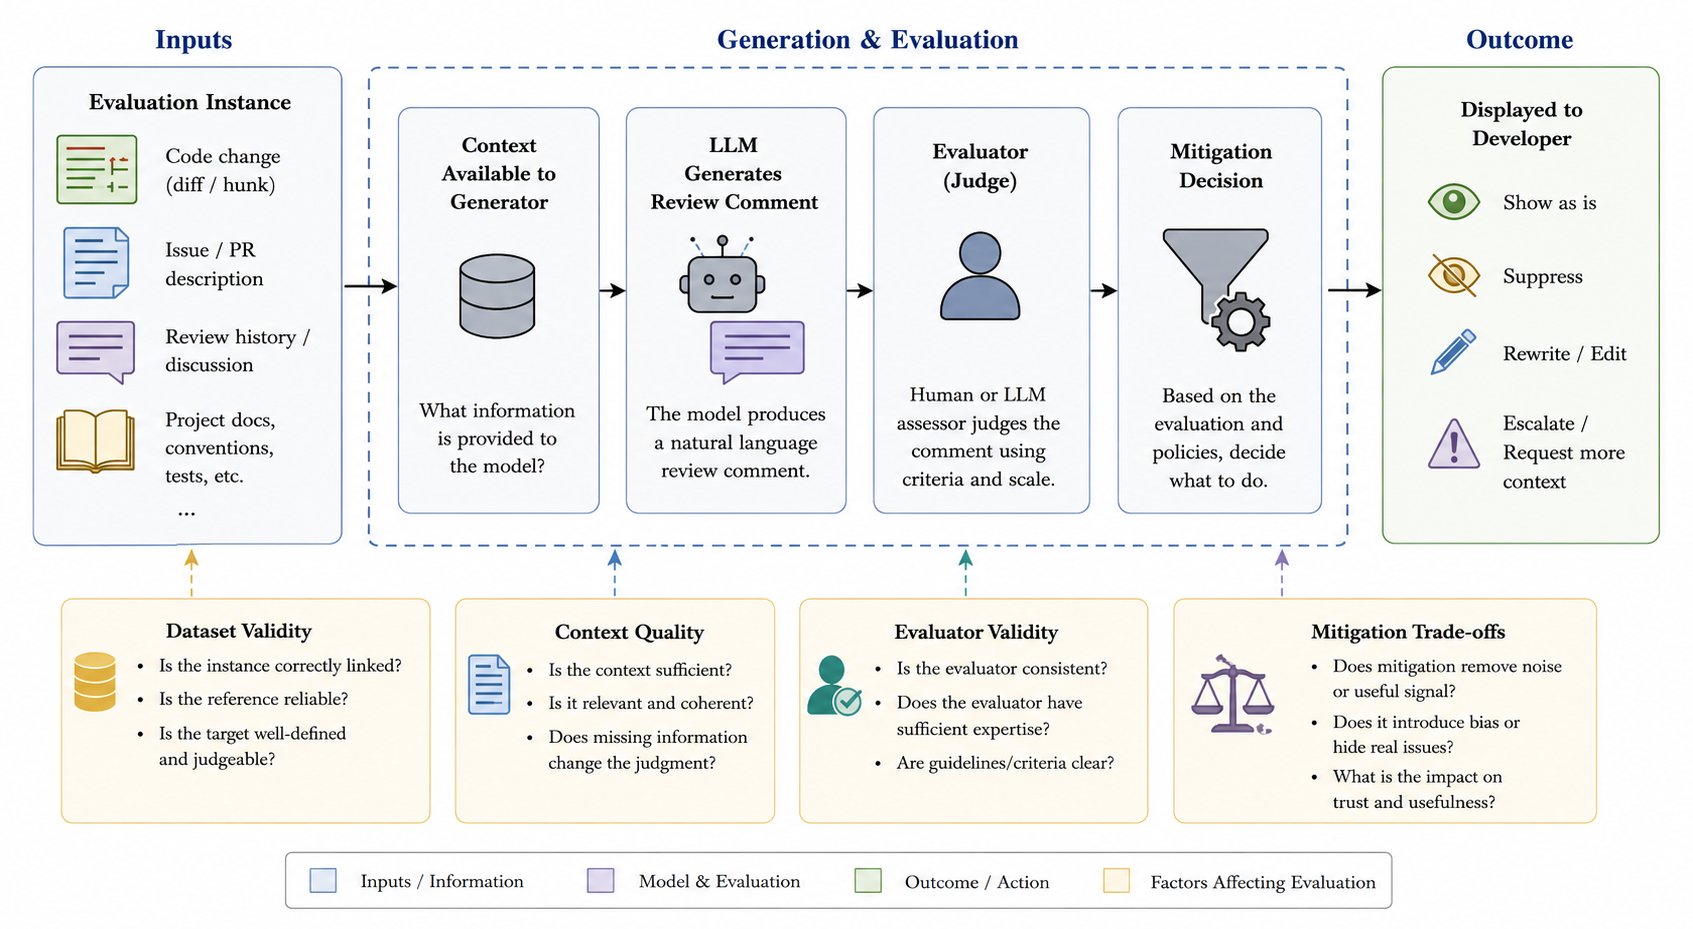
\includegraphics[width=0.95\linewidth]{../figures/evaluation-pipeline-concepts.png}
\caption{Conceptual pipeline for evaluating LLM-generated code review comments. The generated comment is only one part of the evaluation problem: dataset validity, context quality, evaluator validity, and mitigation trade-offs can each affect the final decision.}
\label{fig:evaluation-pipeline-concepts}
\end{figure}

\subsection{Why Generated Review Comments Are Difficult to Evaluate}

Generated review comments are difficult to evaluate because there is rarely a single correct comment for a code change. Human reference comments are useful, but they are incomplete and noisy. Reviewers may focus on different issues, express feedback at different levels of detail, or leave no comment even when a change has reviewable concerns. A generated comment can therefore be useful without matching a reference comment in wording or location \cite{p01_lu2025_deepcrceval,p08_liu2025_too_noisy,p18_bensghaier2025_curated_reviews,p52_tufano2021_automating_code_review_activities,p53_tufano2024_code_review_automation_strengths_weaknesses}.

There is also a quieter failure mode: a generated comment can sound fluent and relevant while having no support in the available context. It may infer a bug that is not present, assume a missing condition that is actually handled elsewhere, propose a fix that does not apply, or point the reviewer to the wrong location. Such comments can consume reviewer attention and reduce trust in the assistant \cite{p02_tantithamthavorn2026_hallujudge,p35_mcaleese2024_llm_critics}.

Usefulness and correctness describe different properties. Correct feedback can be too vague or minor to assist a reviewer, whereas an uncertain observation can still prompt a worthwhile check. Binary correct/incorrect or accepted/rejected labels obscure these cases \cite{p10_sun2025_bitsai_cr,p19_nguyen2025_fine_grained_classification,p39_bosu2015_useful_reviews,p53_tufano2024_code_review_automation_strengths_weaknesses}.

A third difficulty comes from the evaluation instance. In a generation failure, the model produces a poor comment for a valid instance. In a dataset-validity problem, the instance itself does not support a reliable judgment. Mined review data can contain comments that are unclear in the available context, do not request a change, were ignored, or are linked to the wrong code \cite{p52_tufano2021_automating_code_review_activities,p53_tufano2024_code_review_automation_strengths_weaknesses}. Such cases can distort training and evaluation because the target may not represent a judgeable review action.

Evaluator behavior introduces a fourth difficulty. LLM-as-a-Judge assessment can reduce manual effort, but judgments vary with prompts, answer order, model choice, verbosity, and task framing \cite{m04_zheng2023_llm_judge,p29_wang2025_human_evaluators,p31_jiang2025_codejudgebench,p32_zhao2026_bias_loop,p33_he2025_llmjudge_se}. These sensitivities affect construct validity whenever judge outputs support a performance claim.

These distinctions provide the vocabulary used by the taxonomy and the evaluation framework developed later in the paper.



% Source: drafts/paper/sections/03-related-work.md

\section{Related Work}

Research relevant to LLM-based code review spans review automation, benchmarks, grounding and context, human-centered evaluation, mitigation, and evaluator validity. Figure \ref{fig:related-work-coverage-map} shows the concerns emphasized by each stream and the limited overlap among them.

\begin{figure}[H]
\centering
\resizebox{0.98\linewidth}{!}{%
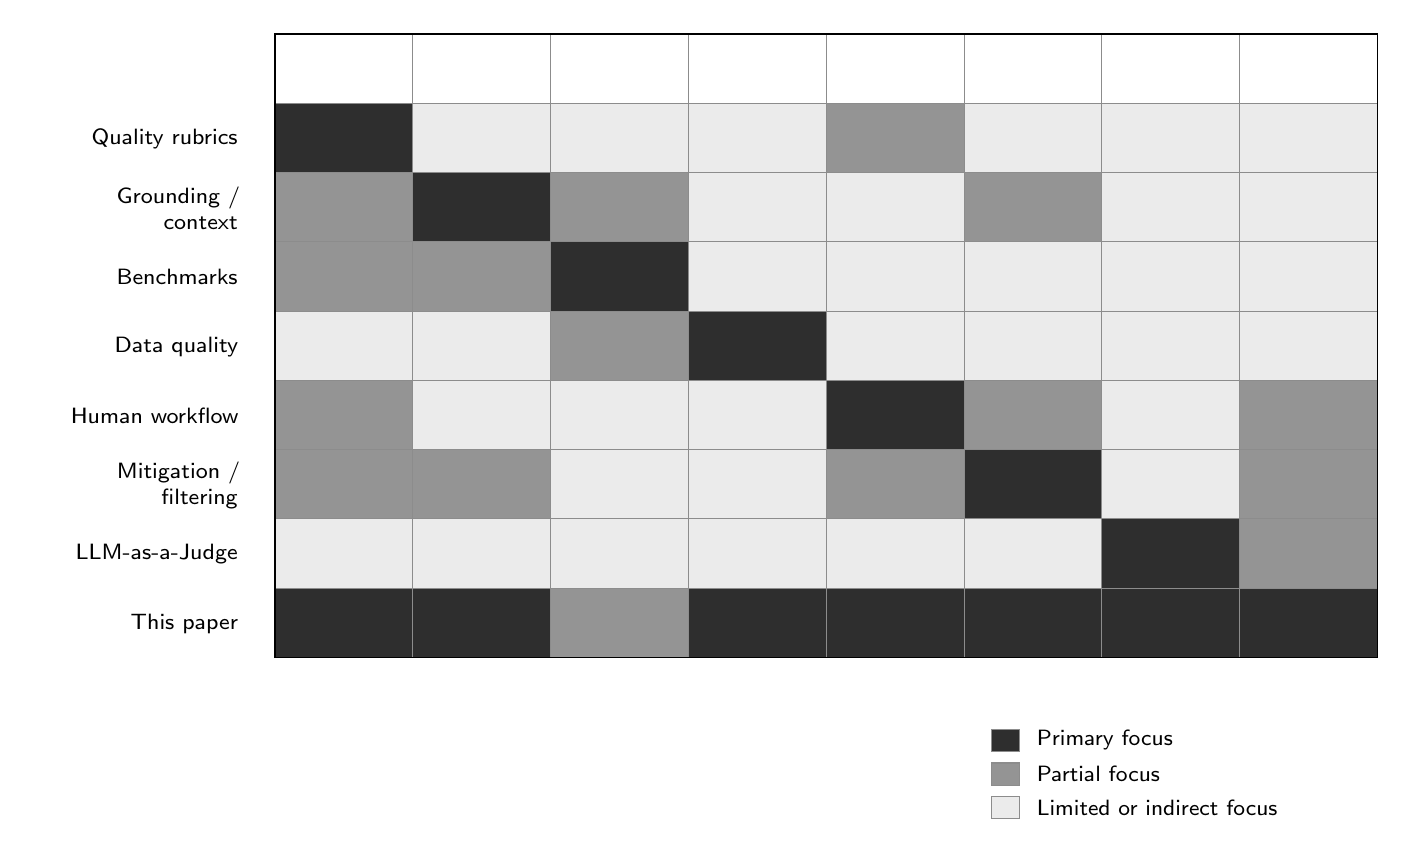
\begin{tikzpicture}[
  font=\sffamily\footnotesize,
  header/.style={font=\sffamily\bfseries\footnotesize, align=center, text width=2.05cm},
  rowlabel/.style={font=\sffamily\footnotesize, align=right, text width=2.55cm},
  celltext/.style={font=\sffamily\scriptsize, align=center},
  legendtext/.style={font=\sffamily\footnotesize, anchor=west},
]

\definecolor{primaryFocus}{gray}{0.18}
\definecolor{partialFocus}{gray}{0.58}
\definecolor{limitedFocus}{gray}{0.92}
\definecolor{gridLine}{gray}{0.55}

\def\cellw{1.75}
\def\cellh{0.88}
\def\xstart{3.0}
\def\ystart{0}

% Column headers.
\node[header] at (3.875, 0.55) {Quality};
\node[header] at (5.625, 0.55) {Grounding};
\node[header] at (7.375, 0.55) {Benchmark\\realism};
\node[header] at (9.125, 0.55) {Data\\validity};
\node[header] at (10.875, 0.55) {Workflow\\value};
\node[header] at (12.625, 0.55) {Mitigation};
\node[header] at (14.375, 0.55) {Evaluator\\validity};
\node[header] at (16.125, 0.55) {Decision\\level};

% Row labels.
\node[rowlabel] at (1.25, -0.45) {Quality rubrics};
\node[rowlabel] at (1.25, -1.33) {Grounding /\\context};
\node[rowlabel] at (1.25, -2.21) {Benchmarks};
\node[rowlabel] at (1.25, -3.09) {Data quality};
\node[rowlabel] at (1.25, -3.97) {Human workflow};
\node[rowlabel] at (1.25, -4.85) {Mitigation /\\filtering};
\node[rowlabel] at (1.25, -5.73) {LLM-as-a-Judge};
\node[rowlabel] at (1.25, -6.61) {This paper};

% Helper macro: x index, y index, color.
\newcommand{\focuscell}[3]{%
  \pgfmathsetmacro{\x}{\xstart + (#1) * \cellw}%
  \pgfmathsetmacro{\y}{\ystart - (#2) * \cellh}%
  \draw[draw=gridLine, line width=0.35pt, fill=#3] (\x,\y) rectangle ++(\cellw,-\cellh);%
}

% Header row cells.
\foreach \c in {0,...,7} {\focuscell{\c}{-1}{white}}

% Row 1: Quality rubrics.
\focuscell{0}{0}{primaryFocus}
\focuscell{1}{0}{limitedFocus}
\focuscell{2}{0}{limitedFocus}
\focuscell{3}{0}{limitedFocus}
\focuscell{4}{0}{partialFocus}
\focuscell{5}{0}{limitedFocus}
\focuscell{6}{0}{limitedFocus}
\focuscell{7}{0}{limitedFocus}

% Row 2: Grounding/context.
\focuscell{0}{1}{partialFocus}
\focuscell{1}{1}{primaryFocus}
\focuscell{2}{1}{partialFocus}
\focuscell{3}{1}{limitedFocus}
\focuscell{4}{1}{limitedFocus}
\focuscell{5}{1}{partialFocus}
\focuscell{6}{1}{limitedFocus}
\focuscell{7}{1}{limitedFocus}

% Row 3: Benchmarks.
\focuscell{0}{2}{partialFocus}
\focuscell{1}{2}{partialFocus}
\focuscell{2}{2}{primaryFocus}
\focuscell{3}{2}{limitedFocus}
\focuscell{4}{2}{limitedFocus}
\focuscell{5}{2}{limitedFocus}
\focuscell{6}{2}{limitedFocus}
\focuscell{7}{2}{limitedFocus}

% Row 4: Data quality.
\focuscell{0}{3}{limitedFocus}
\focuscell{1}{3}{limitedFocus}
\focuscell{2}{3}{partialFocus}
\focuscell{3}{3}{primaryFocus}
\focuscell{4}{3}{limitedFocus}
\focuscell{5}{3}{limitedFocus}
\focuscell{6}{3}{limitedFocus}
\focuscell{7}{3}{limitedFocus}

% Row 5: Human workflow.
\focuscell{0}{4}{partialFocus}
\focuscell{1}{4}{limitedFocus}
\focuscell{2}{4}{limitedFocus}
\focuscell{3}{4}{limitedFocus}
\focuscell{4}{4}{primaryFocus}
\focuscell{5}{4}{partialFocus}
\focuscell{6}{4}{limitedFocus}
\focuscell{7}{4}{partialFocus}

% Row 6: Mitigation/filtering.
\focuscell{0}{5}{partialFocus}
\focuscell{1}{5}{partialFocus}
\focuscell{2}{5}{limitedFocus}
\focuscell{3}{5}{limitedFocus}
\focuscell{4}{5}{partialFocus}
\focuscell{5}{5}{primaryFocus}
\focuscell{6}{5}{limitedFocus}
\focuscell{7}{5}{partialFocus}

% Row 7: LLM-as-a-Judge.
\focuscell{0}{6}{limitedFocus}
\focuscell{1}{6}{limitedFocus}
\focuscell{2}{6}{limitedFocus}
\focuscell{3}{6}{limitedFocus}
\focuscell{4}{6}{limitedFocus}
\focuscell{5}{6}{limitedFocus}
\focuscell{6}{6}{primaryFocus}
\focuscell{7}{6}{partialFocus}

% Row 8: This paper.
\focuscell{0}{7}{primaryFocus}
\focuscell{1}{7}{primaryFocus}
\focuscell{2}{7}{partialFocus}
\focuscell{3}{7}{primaryFocus}
\focuscell{4}{7}{primaryFocus}
\focuscell{5}{7}{primaryFocus}
\focuscell{6}{7}{primaryFocus}
\focuscell{7}{7}{primaryFocus}

% Outer border.
\draw[draw=black, line width=0.6pt] (\xstart,0.88) rectangle ++(8*\cellw,-9*\cellh);

% Legend.
\draw[fill=primaryFocus, draw=gridLine] (12.1,-7.95) rectangle ++(0.35,-0.28);
\node[legendtext] at (12.55,-8.09) {Primary focus};
\draw[fill=partialFocus, draw=gridLine] (12.1,-8.38) rectangle ++(0.35,-0.28);
\node[legendtext] at (12.55,-8.52) {Partial focus};
\draw[fill=limitedFocus, draw=gridLine] (12.1,-8.81) rectangle ++(0.35,-0.28);
\node[legendtext] at (12.55,-8.95) {Limited or indirect focus};

\end{tikzpicture}%
}

\caption{Interpretive coverage map of related literature. Dark marks indicate a primary concern, medium marks a recurring concern, and light marks limited treatment. The marks are qualitative, not frequency estimates or independently coded scores.}
\label{fig:related-work-coverage-map}
\end{figure}

\subsection{Review Automation and Evaluation}

Modern code review supports defect detection as well as maintainability, knowledge transfer, team awareness, and shared ownership \cite{p37_sadowski2018_google_mcr,p38_bacchelli2013_expectations_mcr,p39_bosu2015_useful_reviews,p51_davila2021_mcr_slr_taxonomy}. Automation studies extended this practice by mining review interactions and generating comments or code revisions. They also exposed substantial variation in review intent and artifact quality: mined comments may request changes, explain decisions, discuss design, or provide feedback that is not directly actionable \cite{p14_li2022_codereviewer,p52_tufano2021_automating_code_review_activities,p53_tufano2024_code_review_automation_strengths_weaknesses}. Consequently, resemblance to a reference comment captures only part of review quality.

Evaluation research has responded with review-specific rubrics and more realistic benchmarks. DeepCRCEval distinguishes several dimensions of comment quality, while data-curation and preference studies assess properties such as clarity, conciseness, usefulness, and developer preference \cite{p01_lu2025_deepcrceval,p18_bensghaier2025_curated_reviews,p30_weyssow2025_codeultrafeedback}. PR-level and context-aware benchmarks connect feedback to broader change context, issue coverage, and review comprehension \cite{p04_kumar2026_swe_prbench,p05_zeng2025_swrbench,p06_hu2025_contextcrbench,p17_lin2025_codereviewqa}. Collectively, these studies broaden what is measured, although their constructs and units of analysis remain heterogeneous.

\subsection{Context, Grounding, and Data Validity}

Grounding studies examine whether review claims are supported by the available change and project evidence. Missing information about surrounding code, framework behavior, or configuration can make fluent feedback unreliable \cite{p02_tantithamthavorn2026_hallujudge,p03_tantithamthavorn2026_rovodev,p07_olewicki2024_revmate}. Retrieval, repository-aware analysis, specifications, and static-analysis output can strengthen this evidence base \cite{p11_zhang2025_laura,p12_wang2025_sgcr,p16_icoz2026_context_aware,p20_hong2025_rag_reviewer,p22_jaoua2025_static_analyzers}. Their value depends on relevance and consistency, however. Additional context may distract the model, while retrieved documentation or examples may be stale or contradictory \cite{p04_kumar2026_swe_prbench,p13_haider2024_prompting_finetuning,p40_ram2018_reviewability,p49_lee2025_metamon}. Context availability must therefore be distinguished from context quality and usability.

Training and evaluation data pose a related validity problem. Repository-mined comments can be vague, redundant, uncivil, or detached from the discussion that made them meaningful. Cleaning and reformulation may improve model training while changing intent or removing useful signals \cite{p08_liu2025_too_noisy,p18_bensghaier2025_curated_reviews}. Reference quality also depends on reviewer experience, provenance, judge selection, and labeling procedure \cite{p23_lin2026_reviewer_experience,p30_weyssow2025_codeultrafeedback,p42_wasserbaech2024_chatgpt_github}. An unreliable instance can therefore produce an apparent model error that is better understood as a data or benchmark failure.

\subsection{Human Value and Workflow Evidence}

Industrial and human-centered studies complement offline metrics with perceived value, actionability, reviewer effort, revision behavior, cycle time, and adoption \cite{p03_tantithamthavorn2026_rovodev,p07_olewicki2024_revmate,p10_sun2025_bitsai_cr}. Other work examines how AI involvement changes feedback diversity, review interactions, accountability, learning, and ownership \cite{p26_zhong2026_human_ai_synergy,p27_chowdhury2026_industry_claims,p28_heander2025_support_not_automation}. These studies show why acceptance is an incomplete proxy: rejected feedback may still prompt useful investigation, whereas accepted feedback may be obvious or costly. Workflow outcomes and comment quality should therefore be reported separately.

\subsection{Failure Types and Mitigation}

Generated feedback can fail through unsupported or incorrect claims, misplaced diagnoses, irrelevance, weak explanations, unsafe fixes, or low-value repetition \cite{p01_lu2025_deepcrceval,p02_tantithamthavorn2026_hallujudge,p19_nguyen2025_fine_grained_classification,p25_yu2024_finetuning_acr,p41_widyasari2025_explaining_explanations}. Some apparent failures instead originate in incomplete context, weak references, workflow mismatch, or the evaluator. Specialized settings add domain-specific evidence requirements: security comments need vulnerability and repair validation, static-analysis feedback depends on correct warning interpretation, and performance advice requires representative workloads \cite{p21_peng2025_icodereviewer,p22_jaoua2025_static_analyzers,p46_zhou2025_vulnerability_repair,p48_patcas2026_code_quality_issues,p50_peng2025_coffe}. Distinguishing these causes matters because they call for different interventions.

Mitigation can alter data, context, generation, or post-generation handling. Representative approaches include data curation, retrieval, specification or tool grounding, fine-tuning, critics, filtering, rewriting, and human referral \cite{p08_liu2025_too_noisy,p09_ren2025_hydra_reviewer,p11_zhang2025_laura,p12_wang2025_sgcr,p22_jaoua2025_static_analyzers,p24_bensghaier2025_reward_models,p35_mcaleese2024_llm_critics}. Their evaluations use different outcomes and seldom provide directly comparable accounts of what an intervention retains, removes, or costs.

\subsection{LLM-as-a-Judge Validity}

LLM-as-a-Judge methods offer scalable structured assessment \cite{m04_zheng2023_llm_judge,p29_wang2025_human_evaluators,p31_jiang2025_codejudgebench,p33_he2025_llmjudge_se,p36_li2024_llms_as_judges}. Their decisions can vary with task, prompt, response order, source model, verbosity, and adversarial context \cite{p30_weyssow2025_codeultrafeedback,p32_zhao2026_bias_loop,p63_mitropoulos2026_confirmation_bias,p64_thornton2026_adversarial_comments}. This literature contributes methods for calibration, repeated-run analysis, perturbation testing, and comparison with human judgments.

Taken together, prior work supplies rich but fragmented evidence about comments, inputs, workflows, interventions, and evaluators. This review organizes that evidence around failure diagnosis and the consequences of mitigation, providing the basis for the taxonomy and framework developed below.



% Source: drafts/paper/sections/04-methodology.md

\section{Review Method}

\subsection{Review Design}

We conducted a targeted structured literature review using documented multi-source search streams. The method covers question definition, eligibility assessment, quality appraisal, data extraction, thematic synthesis, and reporting. It draws on software-engineering SLR guidance \cite{m00_kitchenham2007_slr_guidelines}, while taxonomy construction and reliability planning draw on established taxonomy and agreement methods \cite{m01_nickerson2013_taxonomy,m02_cohen1960_kappa,m03_krippendorff2018_content_analysis}.

\subsubsection{Goal definition}

Following a Goal--Question--Metric structure, the review goal is defined as follows:

\begin{itemize}
\item \textbf{Purpose:} analyze and characterize;
\item \textbf{Issue:} evaluation and mitigation trade-offs;
\item \textbf{Object:} LLM-generated and automated code review comments and their evaluation instruments; and
\item \textbf{Viewpoint:} researchers and tool builders designing reliable code-review evaluation.
\end{itemize}

Five review questions refine this goal, while the extraction fields identify the evidence required to answer each question. Framework derivation is treated separately as a traceability objective rather than as a research question, because the framework is an author-derived synthesis artifact.

\subsection{Review Questions}

\begin{table}[H]
\centering
\footnotesize
\renewcommand{\arraystretch}{1.18}
\begin{tabularx}{\linewidth}{@{}>{\raggedright\arraybackslash}p{0.55in}>{\raggedright\arraybackslash}X@{}}
\toprule
\rowcolor{ACMTableHead}
\textbf{RQ} & \textbf{Question} \\
\midrule
RQ1 & Which problematic-comment types and failure categories have been reported? \\
RQ2 & Which evaluation dimensions have been used for correctness, grounding, relevance, usefulness, actionability, context quality, and evaluator validity? \\
RQ3 & Which mitigation families have been proposed or evaluated, and where do they intervene? \\
RQ4 & What evidence exists about error reduction versus useful-feedback preservation, coverage, escalation, and cost? \\
RQ5 & How are context quality, dataset validity, and annotation difficulty treated? \\
\bottomrule
\end{tabularx}
\end{table}

Table \ref{tab:rq-traceability} links each question to its evidence and synthesis path. The unit for all frequency counts is the included study unless a result names a different denominator.

\begingroup
\footnotesize
\renewcommand{\arraystretch}{1.18}
\begin{longtable}{@{}>{\raggedright\arraybackslash}p{0.12\textwidth}>{\raggedright\arraybackslash}p{0.12\textwidth}>{\raggedright\arraybackslash}p{0.12\textwidth}>{\raggedright\arraybackslash}p{0.12\textwidth}>{\raggedright\arraybackslash}p{0.12\textwidth}>{\raggedright\arraybackslash}p{0.12\textwidth}>{\raggedright\arraybackslash}p{0.12\textwidth}@{}}
\caption{Traceability from review questions to evidence and reported outputs.}\label{tab:rq-traceability} \\
\toprule
\rowcolor{ACMTableHead}
\textbf{RQ} & \textbf{Eligibility scope} & \textbf{Extracted fields} & \textbf{Unit of analysis} & \textbf{Synthesis method} & \textbf{Reported output} & \textbf{Principal validity limitation} \\
\midrule
\endfirsthead
\caption[]{Traceability from review questions to evidence and reported outputs. (continued)} \\
\toprule
\rowcolor{ACMTableHead}
\textbf{RQ} & \textbf{Eligibility scope} & \textbf{Extracted fields} & \textbf{Unit of analysis} & \textbf{Synthesis method} & \textbf{Reported output} & \textbf{Principal validity limitation} \\
\midrule
\endhead
\midrule
\multicolumn{7}{r}{Continued on next page} \\
\endfoot
\bottomrule
\endlastfoot
RQ1 & Direct or supporting evidence about problematic review feedback or related failure modes & failure categories, evidence status, evidence location & study-level presence of coded evidence & controlled-vocabulary tabulation and thematic grouping & failure-frequency table and proposed taxonomy & source studies use different labels; comment-level prevalence is not estimated \\
RQ2 & Studies evaluating comment quality, workflow outcomes, context, or evaluator behavior & evaluation dimensions, artifact, context, evaluator type & study-level presence of an evaluated construct & frequency tabulation and construct synthesis & evaluation-dimension table and construct map & definitions and measurement protocols differ across studies \\
RQ3 & Studies proposing or evaluating an intervention relevant to review feedback & mitigation family, intervention point, reported outcomes & study-level presence of a mitigation family & intervention-point classification & mitigation-family table and strategy map & frequency does not establish comparative effectiveness \\
RQ4 & Studies reporting preservation, coverage, escalation, or cost & reporting-availability fields and evidence status & study-level reporting availability within the stated corpus or subset & descriptive counts and sensitivity analysis & trade-off availability and subset tables & missing reporting is not a zero effect; effect sizes are not pooled \\
RQ5 & Studies addressing context, dataset, annotation, or judge validity & context types, data validity, annotation, evaluator-validity evidence & study-level coded evidence and cross-study theme & thematic synthesis and context-frequency tabulation & context-validity synthesis and framework qualifications & coding is single-reviewer and adjacent evidence requires transfer judgment \\
\end{longtable}
\endgroup

\subsubsection{Framework-traceability objective}

For each taxonomy category, annotation decision, and framework layer, we record whether support is direct code-review evidence, supporting evidence, or a bounded transfer from peripheral evidence. This mapping documents derivation; it is not treated as independent validation of the proposed framework.

\subsection{Search Scope and Corpus Assembly}

The review protocol identified ACM Digital Library, IEEE Xplore, ScienceDirect, SpringerLink, arXiv, Semantic Scholar, Google Scholar, and Scopus where available, with a primary focus on work from 2021 onward and earlier foundational modern-code-review studies. Query families covered LLM code review, automated review, generated comments, evaluation metrics, hallucination and grounding, context-aware review, LLM-as-a-Judge, and human--AI review. Complete screenable result sets were retained for every planned source except Scopus, which was formally closed because neither authenticated API access nor institutional document-search access was available. This access limitation is not interpreted as a zero-result search.

The synthesis corpus contains 121 unique full-text studies identified across arXiv, OpenAlex, Crossref, publisher indexes, and general scholarly-web search. Separate topic families covered direct code review, generated comments, evaluator validity, modern code review, surveys, security, refinement, efficiency, and industrial evidence. Every included study was verified as retrievable through at least one topic-level query without using its title, identifier, system name, or author name as the query. All included studies subsequently underwent the same eligibility, extraction, evidence-tier, and appraisal procedure.

The later multi-source reconciliation produced a separate pool of 1,358 unique candidate identities, including 1,348 candidates not matched to the frozen corpus. These candidates remain search and screening artifacts rather than included studies: DOI enrichment and title/abstract triage do not establish eligibility, full-text inclusion, or extraction completeness. Their metadata are retained in the replication package for auditability, but they are not counted in any RQ denominator and are not displayed as article references in the PDF.

\subsubsection{Search execution and corpus closure}

The principal reproducible run began with arXiv because its public API returned exact-query results and stable retrieval counts. Topic-level searches in OpenAlex, Crossref, publisher indexes, and the scholarly web broadened coverage for adjacent and foundational evidence. Semantic Scholar was initially rate-limited, but a rate-limited bulk-API rerun completed on 6 August 2026. Because the API does not accept the protocol's nested Boolean expression directly, the two concept blocks were expanded into 16 phrase-level conjunctions (four LLM terms crossed with four review terms), and results were deduplicated by Semantic Scholar paper identifier. Manual authorised-browser runs subsequently retained complete screenable sets from ACM Digital Library, IEEE Xplore, ScienceDirect, SpringerLink, and Google Scholar. These later sets remain outside the frozen synthesis denominator until title/abstract screening, full-text assessment, and cross-source identity reconciliation are complete.

The arXiv search was executed on 2 August 2026 for records submitted from 1 January 2021 through 2 August 2026. Table \ref{tab:arxiv-queries} reports the exact API queries. The raw API responses and screening decisions were retained during the review process but are not included with this PDF.

\begin{table}[H]
\centering
\caption{Exact queries used in the reproducible arXiv search stream.}
\label{tab:arxiv-queries}
\footnotesize
\renewcommand{\arraystretch}{1.18}
\begin{tabularx}{\linewidth}{@{}>{\raggedright\arraybackslash}p{0.9in}>{\raggedright\arraybackslash}X@{}}
\toprule
\rowcolor{ACMTableHead}
\textbf{Query (retrieved)} & \textbf{Exact arXiv query} \\
\midrule
Q1 (200) & \texttt{(ti:"code review" OR abs:"code review") AND (ti:"large language model" OR abs:"large language model" OR ti:LLM OR abs:LLM) AND submittedDate:[202101010000 TO 202608022359]} \\
Q2 (61) & \texttt{(ti:"review comment" OR abs:"review comment") AND (ti:"large language model" OR abs:"large language model" OR ti:LLM OR abs:LLM) AND submittedDate:[202101010000 TO 202608022359]} \\
Q3 (156) & \texttt{(ti:"code review" OR abs:"code review") AND (all:hallucination OR all:grounding OR all:context) AND submittedDate:[202101010000 TO 202608022359]} \\
\bottomrule
\end{tabularx}
\end{table}

Table \ref{tab:source-search-status} reports the execution status of every source named in the protocol through 6 August 2026. Blank counts denote unavailable result sets, not zero results.

\begin{table}[H]
\centering
\caption{Execution status of the planned search sources through 6 August 2026.}
\label{tab:source-search-status}
\footnotesize
\renewcommand{\arraystretch}{1.18}
\begin{tabularx}{\linewidth}{@{}>{\raggedright\arraybackslash}p{0.23\linewidth}>{\raggedright\arraybackslash}X>{\raggedright\arraybackslash}X@{}}
\toprule
\rowcolor{ACMTableHead}
\textbf{Source} & \textbf{Exact executed or attempted query} & \textbf{Result status} \\
\midrule
arXiv & Q1--Q3 in Table \ref{tab:arxiv-queries} & Complete retained run: 417 raw, 293 unique \\
Semantic Scholar & 16 pairwise bulk-API queries: each of \texttt{\{"large language model", LLM, "generative AI", "AI-assisted"\}} combined with each of \texttt{\{"code review", "review comment", "pull request feedback", "automated code review"\}} & Complete retained run on 6 August 2026: 963 raw, 427 unique \\
ACM Digital Library & \texttt{"large language model" AND "code review"} & Complete manual-browser run: 449 results and 449 unique record URLs \\
IEEE Xplore & \texttt{"large language model" AND "code review"}, years 2021--2026 & Complete retained browser run on 6 August 2026: 69 results \\
ScienceDirect & \texttt{"large language model" AND "code review"}, years 2021--2026 & Complete manual-browser run: 318 results and 318 unique PII record URLs \\
SpringerLink & \texttt{"large language model" AND "code review"}, years 2021--2026, English & Complete native CSV export: 155 results and 155 unique DOIs \\
Google Scholar & \texttt{"large language model" AND "code review"}, date sorting & Complete exposed manual-browser set: approximately 81 reported results and 81 unique Scholar identifiers \\
Scopus & \texttt{TITLE-ABS-KEY("large language model" AND "code review")} with years 2021--2026 & Formally closed: API unavailable and Scopus Preview did not expose document search or export \\
\bottomrule
\end{tabularx}
\end{table}

The retained partial export contained 38 source rows from ACM Digital Library, IEEE Xplore, ScienceDirect, SpringerLink, and Semantic Scholar, which reconciled to 30 candidate records. Because native totals and complete result sets were unavailable, this export is a cross-check rather than a reproducible database-search denominator.

The three result sets contained 417 raw records. Deduplication by arXiv identifier removed 124 cross-query repetitions while preserving every matching query identifier, leaving 293 unique records. Conservative title/abstract screening assigned one of four outcomes: include for full text, exclude, duplicate/companion, or uncertain. The controlled exclusion vocabulary was \texttt{out of scope}, \texttt{no review-feedback connection}, \texttt{insufficient method/evaluation}, \texttt{duplicate/companion}, \texttt{non-English}, \texttt{inaccessible}, and \texttt{supporting-only methodology}. This stage retained 140 records for full-text assessment, excluded 116, and identified 37 duplicate or likely companion records.

Full-text inclusion required a recorded decision, inclusion group, eligibility criterion, evidence location, rationale, reviewer, and screening date. Of the 140 records assessed in the arXiv stream, 132 were retained for consideration and eight were excluded. Fifty-three retained records met core criteria; identity reconciliation found one overlap with the existing candidate pool and two duplicate or companion identities. A candidate entered the final corpus only after its identity, eligibility decision, evidence record, and bibliographic entry were complete.

The remaining 79 records form the supporting reserve: 53 have substantive provisional extraction, 16 have scaffolds only, and ten have no extraction packet. They are not included in the 121-study denominator. Inaccessible records without enough evidence for classification were excluded; seven access-limited records from the later external export remain metadata-only and outside the frozen corpus.

An external 30-record export was screened separately after corpus closure. Reconciliation found 20 duplicates, two full-text candidates retained outside the closed corpus, seven access-limited metadata-only candidates, and one exclusion. The external export therefore contributes no study to the 121-study denominator. The two eligible full-text candidates were not incorporated because the corpus had already been frozen, but corpus closure was not specified prospectively. Their exclusion is therefore a post hoc boundary and a threat to selection validity. Candidate-level decisions are retained in the replication package.

\begingroup
\footnotesize
\renewcommand{\arraystretch}{1.18}
\begin{longtable}{@{}>{\raggedright\arraybackslash}p{0.15\textwidth}>{\raggedright\arraybackslash}p{0.17\textwidth}>{\raggedright\arraybackslash}p{0.19\textwidth}>{\raggedright\arraybackslash}p{0.23\textwidth}>{\raggedright\arraybackslash}p{0.18\textwidth}@{}}
\caption{Accounting of the unified corpus and auxiliary candidate sets.}\label{tab:corpus-flow-audit} \\
\toprule
\rowcolor{ACMTableHead}
\textbf{Record set} & \textbf{Identified or retained} & \textbf{Full text assessed} & \textbf{Included in synthesis corpus} & \textbf{Outside corpus} \\
\midrule
\endfirsthead
\caption[]{Accounting of the unified corpus and auxiliary candidate sets. (continued)} \\
\toprule
\rowcolor{ACMTableHead}
\textbf{Record set} & \textbf{Identified or retained} & \textbf{Full text assessed} & \textbf{Included in synthesis corpus} & \textbf{Outside corpus} \\
\midrule
\endhead
\midrule
\multicolumn{5}{r}{Continued on next page} \\
\endfoot
\bottomrule
\endlastfoot
Unified synthesis corpus & 121 & 121 & 121 & 0 \\
Reproducible arXiv stream & 293 unique & 140 & Reconciled into unified corpus & 79 supporting-reserve records \\
External cross-check export & 30 & 3 & Reconciled into unified corpus & 2 post-closure candidates; 20 duplicates; 7 access-limited; 1 exclusion \\
\end{longtable}
\endgroup

The rows are not additive because the search streams overlap and are reconciled by study identity. The synthesis denominator is the 121 unique studies that passed the unified eligibility and extraction procedure.

Figure \ref{fig:corpus-assembly-flow} summarizes the unified corpus assembly and the auxiliary records retained outside its denominator.

\begin{figure}[H]
\centering
\definecolor{flowblue}{RGB}{38,87,139}
\definecolor{flowlight}{RGB}{238,244,251}
\definecolor{flowside}{RGB}{247,247,247}

\resizebox{0.94\linewidth}{!}{%
\begin{tikzpicture}[
  font=\sffamily,
  >=Latex,
  main/.style={draw=flowblue, fill=flowlight, rounded corners=3pt,
    minimum width=4.6cm, minimum height=0.72cm, align=center,
    font=\sffamily\small},
  side/.style={draw=gray!65, fill=flowside, rounded corners=3pt,
    minimum width=3.8cm, minimum height=0.72cm, align=center,
    font=\sffamily\small},
  result/.style={draw=flowblue, fill=flowblue, text=white, rounded corners=3pt,
    minimum width=5.2cm, minimum height=0.82cm, align=center,
    font=\sffamily\small\bfseries},
  arrow/.style={->, draw=gray!75, line width=0.65pt},
  sidearrow/.style={->, dashed, draw=gray!70, line width=0.6pt}
]

\node[main] (raw) {arXiv amendment\\417 raw results};
\node[main, below=0.38cm of raw] (unique) {293 unique records\\after identifier deduplication};
\node[main, below=0.38cm of unique] (full) {140 full texts assessed};
\node[main, below=0.38cm of full] (core) {53 core candidates};
\node[main, below=0.38cm of core] (overlap) {3 overlapping or companion\\identities removed};
\node[main, below=0.38cm of overlap] (added) {50 unique studies added};
\node[result, below=0.64cm of added] (final) {Final synthesis corpus\\121 studies};

\node[side, left=1.25cm of final] (baseline) {Historical baseline\\71 studies\\identification flow not retained};
\node[side, right=1.25cm of full] (reserve) {Supporting reserve\\79 records\\outside synthesis denominator};
\node[side, right=1.25cm of overlap] (cross) {External cross-check\\30 records\\no corpus additions};

\draw[arrow] (raw) -- (unique);
\draw[arrow] (unique) -- (full);
\draw[arrow] (full) -- (core);
\draw[arrow] (core) -- (overlap);
\draw[arrow] (overlap) -- (added);
\draw[arrow] (added) -- (final);
\draw[arrow] (baseline.east) -- (final.west);
\draw[sidearrow] (full.east) -- (reserve.west);
\draw[sidearrow] (cross.west) -- (overlap.east);

\end{tikzpicture}%
}

\caption{Unified corpus assembly. Overlapping multi-source search streams were reconciled into 121 included studies; the supporting reserve and external cross-check remain outside the synthesis denominator.}
\label{fig:corpus-assembly-flow}
\end{figure}

\subsection{Eligibility and Evidence Tiers}

Core eligibility covered LLM-based, AI-assisted, or automated code review; generated review comments or PR feedback; code-review benchmarks and rubrics; relevant failure types; and mitigation through prompting, filtering, retrieval, verification, tool support, rewriting, or escalation. Supporting eligibility covered evaluator validity, human review, workflow value, annotation, context quality, and methodological foundations. General code generation or repair without a review connection was excluded unless retained as explicitly bounded peripheral evidence.

The synthesis corpus assigns 91 studies to the core tier, 24 to supporting evidence, and six to peripheral evidence. These tiers indicate argumentative role, not methodological quality. The 24 supporting studies in the corpus completed the same structured extraction as the core studies. The 79 reserve studies did not: 53 have substantive but provisional packets, 16 have scaffolds only, and ten lack packets. Mixing this partial coding with standardized study records would make quantitative counts non-comparable. Their exclusion is therefore based on extraction completeness rather than timing alone.

\subsection{Quality Appraisal}

The quality-appraisal instrument contains 12 criteria scored from 0 (\texttt{not reported}) to 2 (\texttt{clearly reported}). The complete definitions, scoring rules, and interpretation limits are provided in the supplementary rubric. Its final calibration on 1 August 2026 separated review relevance, trade-off reporting, workflow consequences, and evaluator validity. All 121 included studies were scored with this same instrument, yielding a maximum of 24 points. Criterion-level scores and evidence notes are retained in the study records. The total is descriptive and does not represent a validated quality scale or an inclusion threshold.

Because the final categories were calibrated during review preparation, we retain criterion-level evidence and do not use the total score as a mechanical inclusion threshold. Evidence tier and confidence remain separate from methodological appraisal.

\subsection{Data Extraction}

Each included study has one structured extraction record derived from its available full text. Records contain bibliographic identity, screening decision, study design, RQ1--RQ5 evidence, traceability, quality appraisal, trade-off and evaluator-validity fields, evidence locations, and unresolved verification items. All 121 records pass the same completeness check. Extraction was performed by one reviewer; the validator checks required fields and controlled values but does not test whether another reviewer would make the same judgments.

Independent agreement was not measured. A future validation step should assign a random 10--20\% sample to a second reviewer for blind eligibility screening and extraction of the principal fields. It should report raw agreement and Cohen's kappa for inclusion decisions, and Krippendorff's alpha for the core failure label, usefulness, actionability, context quality, and handling decision. Disagreements should be adjudicated before any revised rules are applied to affected records. This procedure is proposed future work, not part of the completed review.

\begingroup
\footnotesize
\renewcommand{\arraystretch}{1.18}
\begin{longtable}{@{}>{\raggedright\arraybackslash}p{0.22\textwidth}>{\raggedright\arraybackslash}p{0.34\textwidth}>{\raggedright\arraybackslash}p{0.34\textwidth}@{}}
\caption{Study-level data items and their use in the review.}\label{tab:data-items} \\
\toprule
\rowcolor{ACMTableHead}
\textbf{Data-item group} & \textbf{Fields} & \textbf{Use} \\
\midrule
\endfirsthead
\caption[]{Study-level data items and their use in the review. (continued)} \\
\toprule
\rowcolor{ACMTableHead}
\textbf{Data-item group} & \textbf{Fields} & \textbf{Use} \\
\midrule
\endhead
\midrule
\multicolumn{3}{r}{Continued on next page} \\
\endfoot
\bottomrule
\endlastfoot
Bibliographic & study identity, title, year, venue, publication type & Corpus demographics \\
Evidence weighting & evidence tier, decision, relevance, quality score, confidence & Framework traceability and validity \\
Review artifact & context types, evaluated artifact, evaluator types & RQ2 and RQ5 \\
Failure coding & problematic-comment and related failure categories & RQ1 \\
Evaluation coding & quality, workflow, cost, and evaluator-validity dimensions & RQ2 \\
Mitigation coding & family and intervention point & RQ3 \\
Trade-off reporting & preservation, coverage, escalation, and cost availability & RQ4 \\
Method validity & annotation, limitations, and RQ evidence status & RQ5 and framework traceability \\
\end{longtable}
\endgroup

The main field definitions and controlled labels used in the synthesis are described in the manuscript.

\subsection{Synthesis}

We used tabulation, thematic grouping, and framework mapping. We did not pool incompatible metrics. Initial categories were derived during cross-study synthesis and normalized into controlled vocabularies for failure types, evaluation dimensions, mitigation families, and context types. A deterministic transformation procedure produced one study-level record per included study, retained multi-valued controlled labels, and used \texttt{NR} when the extraction did not contain enough evidence. The resulting counts therefore describe coded evidence in the reviewed studies, not the prevalence of failures in deployed systems.

Consistency checks ensured that each included study occurred once, evidence tiers did not overlap, included studies received the intended tier, citations resolved, and appraisal scores were available. Findings were organized by research question. Every reported count uses the 121-study evidence pool as its denominator unless another denominator is stated.

\subsubsection{Supporting-reserve sensitivity analysis}

We separately mapped the bounded synthesis claims in the 53 substantively extracted reserve packets to five framework-level themes defined before the mapping: evaluation or evaluator validity, context or grounding quality, annotation or dataset validity, human-review or workflow value, and trade-off or mitigation design. This directional analysis asks whether the reserve would require a new top-level component for RQ2, RQ5, or framework traceability. It does not compare effect sizes or add reserve records to the 121-study frequency tables. All 53 packets mapped to at least one existing theme: 26 to evaluation or evaluator validity, 25 to context or grounding quality, two to annotation or dataset validity, 29 to human-review or workflow value, and 23 to trade-off or mitigation design. No new top-level component was required. Because the mapping was conducted by the same reviewer and 26 reserve candidates lack substantive extraction, this result provides a bounded robustness check rather than evidence that the reserve cannot alter lower-level categories or relative emphasis.

\subsection{Protocol Consolidation}

The search documentation was consolidated retrospectively; however, all included studies were subsequently verified against the unified eligibility, extraction, and appraisal procedure. The 12-item appraisal instrument was finalized during extraction calibration on 1 August 2026, before the standardized corpus-wide scoring pass. Evidence-tier assignment distinguishes direct from supporting and peripheral evidence. Seven otherwise relevant records remain outside the frozen corpus because verified full text was unavailable. Any future search rerun will be dated and reported as an update to the consolidated protocol. RQ4 separates quantitative measurement, qualitative evaluation, limitation/design mention, and review inference; only the first two are treated as measured or evaluated evidence.



% Source: drafts/paper/sections/07-illustrative-study.md

\section{Study Selection and Characteristics}

\subsection{Corpus Accounting}

The evidence pool contains 121 unique full-text studies. Each study has one structured extraction record and one bibliographic identity. Duplicate representations were reconciled before analysis, and all records passed the same completeness check.

\begin{table}[H]
\centering
\footnotesize
\renewcommand{\arraystretch}{1.18}
\begin{tabularx}{\linewidth}{@{}>{\raggedright\arraybackslash}p{0.38\linewidth}>{\raggedright\arraybackslash}X@{}}
\toprule
\rowcolor{ACMTableHead}
\textbf{Corpus property} & \textbf{Value} \\
\midrule
Included full-text studies & 121 \\
Core evidence & 91 \\
Supporting evidence & 24 \\
Peripheral evidence & 6 \\
Methodological anchors outside the substantive corpus & 4 \\
Unresolved duplicate study identities & 0 \\
\bottomrule
\end{tabularx}
\end{table}

These counts describe the unified synthesis corpus rather than additive database-search totals. Search-stream records overlap and were reconciled by study identity before the 121-study denominator was frozen.

All counts in this section use the study as the unit of analysis. Percentages use the row-specific study count shown in the corresponding table; none is a comment-level prevalence estimate.

\subsection{Research Streams}

The corpus spans six overlapping streams:

\begin{enumerate}
\item generated review-comment models and datasets;
\item PR-level and context-aware benchmarks;
\item data curation, taxonomy, relevance, and usefulness;
\item industrial and human--AI workflow evidence;
\item LLM-as-a-Judge and evaluator-validity studies; and
\item specialized security, static-analysis, context-consistency, and non-functional evidence.
\end{enumerate}

The first four streams provide the strongest direct evidence for review-comment evaluation. Evaluator studies primarily qualify measurement claims. Specialized and adjacent studies contribute optional sublayers and transfer risks.

\subsection{Publication Demographics}

The corpus is recent: 95 of 121 records (78.5\%) are dated 2025 or 2026. This concentration reflects rapid growth in LLM-based review research, but it also means that many records are recent preprints whose metadata or peer-review status may change.

\begin{table}[H]
\centering
\caption{Distribution of the 121 records by publication period.}
\label{tab:publication-years}
\footnotesize
\renewcommand{\arraystretch}{1.18}
\begin{tabularx}{\linewidth}{@{}>{\raggedright\arraybackslash}p{0.23\linewidth}>{\raggedright\arraybackslash}X>{\raggedright\arraybackslash}X@{}}
\toprule
\rowcolor{ACMTableHead}
\textbf{Publication period} & \textbf{Studies} & \textbf{Share} \\
\midrule
2013--2018 & 4 & 3.3\% \\
2021--2023 & 7 & 5.8\% \\
2024 & 15 & 12.4\% \\
2025 & 49 & 40.5\% \\
2026 & 46 & 38.0\% \\
\bottomrule
\end{tabularx}
\end{table}

The bibliography classifies 44 records as conference papers, 25 as journal articles, and 52 as preprints or other publication forms. Publication type is descriptive and is not used as an inclusion or quality criterion.

\subsection{Appraisal Profile}

All 121 records have Q1--Q12 scores. The mean is 19.90/24, with a range from 12 to 24. This total combines reporting transparency, methodological information, trade-off reporting, and direct relevance to the review. It must therefore not be interpreted as a general measure of methodological quality. Mean scores differ by evidence tier partly because Q12 rewards direct support for this review, not necessarily because adjacent studies use weaker methods.

\begin{table}[H]
\centering
\caption{Mean appraisal score by evidence tier. The score combines reporting and review-specific relevance and is not a general study-quality measure.}
\label{tab:quality-tier}
\footnotesize
\renewcommand{\arraystretch}{1.18}
\begin{tabularx}{\linewidth}{@{}>{\raggedright\arraybackslash}p{0.23\linewidth}>{\raggedright\arraybackslash}X>{\raggedright\arraybackslash}X@{}}
\toprule
\rowcolor{ACMTableHead}
\textbf{Evidence tier} & \textbf{Studies} & \textbf{Mean appraisal score} \\
\midrule
Core & 91 & 20.57/24 \\
Supporting & 24 & 18.67/24 \\
Peripheral & 6 & 14.67/24 \\
Overall & 121 & 19.90/24 \\
\bottomrule
\end{tabularx}
\end{table}

\subsection{Sensitivity Analysis}

We repeated the RQ4 reporting-availability counts for prespecified corpus subsets. To avoid selecting studies partly on the same reporting fields examined by RQ4, the RQ4-independent appraisal subset excludes Q10 (trade-off measurement) and Q12 (direct review support) and retains Q1--Q9 plus Q11. Its threshold is at least 17/20; this threshold is descriptive rather than an inclusion rule. The peer-reviewed subset includes records classified as conference or journal articles. Removing supporting and peripheral studies does not change the four RQ4 numerators because all coded preservation, coverage, escalation, and cost evidence occurs in the core tier. Restricting by publication status or RQ4-independent reporting and methodological appraisal lowers the numerators, but the reporting asymmetry remains.

\begingroup
\footnotesize
\renewcommand{\arraystretch}{1.18}
\begin{longtable}{@{}>{\raggedright\arraybackslash}p{0.18\textwidth}>{\raggedright\arraybackslash}p{0.09\textwidth}>{\raggedright\arraybackslash}p{0.14\textwidth}>{\raggedright\arraybackslash}p{0.13\textwidth}>{\raggedright\arraybackslash}p{0.15\textwidth}>{\raggedright\arraybackslash}p{0.13\textwidth}@{}}
\caption{Sensitivity of RQ4 reporting availability to corpus composition.}\label{tab:sensitivity-rq4} \\
\toprule
\rowcolor{ACMTableHead}
\textbf{Analysis set} & \textbf{Studies} & \textbf{Useful feedback} & \textbf{Coverage} & \textbf{Escalation} & \textbf{Cost} \\
\midrule
\endfirsthead
\caption[]{Sensitivity of RQ4 reporting availability to corpus composition. (continued)} \\
\toprule
\rowcolor{ACMTableHead}
\textbf{Analysis set} & \textbf{Studies} & \textbf{Useful feedback} & \textbf{Coverage} & \textbf{Escalation} & \textbf{Cost} \\
\midrule
\endhead
\midrule
\multicolumn{6}{r}{Continued on next page} \\
\endfoot
\bottomrule
\endlastfoot
All included studies & 121 & 45 (37.2\%) & 46 (38.0\%) & 27 (22.3\%) & 34 (28.1\%) \\
Core evidence only & 91 & 45 (49.5\%) & 46 (50.5\%) & 27 (29.7\%) & 34 (37.4\%) \\
Peer-reviewed only & 69 & 19 (27.5\%) & 20 (29.0\%) & 10 (14.5\%) & 15 (21.7\%) \\
RQ4-independent appraisal at least 17/20 & 77 & 34 (44.2\%) & 34 (44.2\%) & 18 (23.4\%) & 27 (35.1\%) \\
\end{longtable}
\endgroup

\subsection{Evidence Weighting}

Appraisal score and evidence tier are used together. A supporting or peripheral study is not promoted to direct evidence because it has a high appraisal score, and a direct study is not excluded solely because some reporting criteria are weak. Where a paper does not report useful-feedback preservation, escalation, or cost, the absence is coded as missing evidence rather than interpreted as zero impact.

\subsection{Traceability}

The bibliography provides the complete references for the 121 included studies. The paper reports the corpus accounting, evidence tiers, and synthesis procedure, but the study-level extraction records are not included with the standalone PDF.



% Source: drafts/paper/sections/08-findings.md

\section{Results}

The results describe evidence coverage and reporting within the 121-study corpus. Unless stated otherwise, each count is the number of included studies with coded evidence for a field. These study counts do not estimate comment-level prevalence or comparative effects. The current RQ4 fields identify broad reporting availability and do not yet separate quantitative measurement, qualitative evaluation, limitation mentions, and review inference at study level. The corresponding counts are therefore described as mentions or coded evidence, not as measurement frequencies. Missing reporting is not interpreted as a zero effect.

\subsection{RQ1: Problematic-comment Types}

The literature does not support treating all weak comments as hallucinations. Reported failures include unsupported or context-misaligned claims, incorrect technical claims, wrong location or cause, irrelevance, vagueness, non-actionability, invalid fixes, redundancy, low-value nitpicks, severity miscalibration, and context-dependent cases \cite{p02_tantithamthavorn2026_hallujudge,p19_nguyen2025_fine_grained_classification,p21_peng2025_icodereviewer,p58_jin2026_reliable_code_reviewers}. The synthesis further separates input/context failures, workflow failures, and evaluator failures because these require different remedies.

Study-level coding found the broadest evidence coverage for incorrect claims (25 studies), irrelevance (23), spurious or false-positive findings (16), low-value or nitpick feedback (14), unsupported or hallucinated claims (13), and vague or generic feedback (12).

\begin{table}[H]
\centering
\caption{Most frequently coded problematic-comment or related failure categories.}
\label{tab:rq1-failures}
\footnotesize
\renewcommand{\arraystretch}{1.18}
\begin{tabularx}{\linewidth}{@{}>{\raggedright\arraybackslash}p{0.38\linewidth}>{\raggedright\arraybackslash}X@{}}
\toprule
\rowcolor{ACMTableHead}
\textbf{Failure category} & \textbf{Studies with coded evidence} \\
\midrule
Incorrect claim & 25 \\
Irrelevant & 23 \\
Spurious or false positive & 16 \\
Low-value or nitpick & 14 \\
Unsupported or hallucinated & 13 \\
Vague or generic & 12 \\
Missed issue or false negative & 6 \\
Adversarial or biased judgment & 5 \\
\bottomrule
\end{tabularx}
\end{table}

\subsection{RQ2: Evaluation Dimensions}

Evaluation has moved beyond BLEU and exact matching toward semantic, human-centered, and workflow dimensions \cite{p01_lu2025_deepcrceval,p14_li2022_codereviewer,p69_jiang2025_deep_assessment_crg}. However, correctness, grounding, relevance, usefulness, actionability, explanation quality, acceptance, and downstream revision remain distinct constructs. Relevance labels do not establish correctness, and direct acceptance can underestimate perceived value \cite{p07_olewicki2024_revmate,p39_bosu2015_useful_reviews,p57_heumuller2025_relevance_reviews,p60_ahmed2025_feedback_useful}. No single metric in the corpus captures comment quality, coverage, workflow value, and evaluator validity together.

Coverage appears in 28 coded records, followed by lexical similarity (23), evaluator validity and usefulness (22 each), correctness and cost/latency (19 each), and acceptance/adoption (14). Grounding is explicitly coded in four records, even though grounding-related failures occur elsewhere. This difference illustrates why failure categories and evaluation dimensions must be extracted separately.

\begin{table}[H]
\centering
\caption{Most frequently coded evaluation dimensions.}
\label{tab:rq2-dimensions}
\footnotesize
\renewcommand{\arraystretch}{1.18}
\begin{tabularx}{\linewidth}{@{}>{\raggedright\arraybackslash}p{0.38\linewidth}>{\raggedright\arraybackslash}X@{}}
\toprule
\rowcolor{ACMTableHead}
\textbf{Evaluation dimension} & \textbf{Studies with coded evidence} \\
\midrule
Coverage & 28 \\
Lexical similarity & 23 \\
Evaluator validity & 22 \\
Usefulness & 22 \\
Correctness & 19 \\
Cost or latency & 19 \\
Acceptance or adoption & 14 \\
Workflow impact & 12 \\
Explanation quality & 11 \\
\bottomrule
\end{tabularx}
\end{table}

\subsection{RQ3: Mitigation Families}

Mitigations intervene before generation, during generation, after generation, or before display. Pre-generation approaches include data cleaning, reviewability or context gates, and context selection. Generation-time approaches include prompting, fine-tuning, retrieval, specification grounding, static-analysis support, routing, and multi-agent generation. Post-generation approaches include critics, grounding checks, relevance or actionability filters, repair validation, rewriting, aggregation, and staged verification. Pre-display decisions include suppression and human escalation \cite{p08_liu2025_too_noisy,p10_sun2025_bitsai_cr,p11_zhang2025_laura,p35_mcaleese2024_llm_critics}.

Filtering/suppression is the most frequently coded family (30 studies), followed by human escalation (27), fine-tuning (20), verification/critics (15), retrieval/RAG (14), and prompting (11). Benchmark/rubric interventions appear in ten studies. Less frequent families include data cleaning, reward optimization, rewriting, static-analysis hybrids, multi-agent generation, specification grounding, and routing. Frequency does not establish effectiveness because the studies use different artifacts and outcomes.

\begin{table}[H]
\centering
\caption{Most frequently coded mitigation families.}
\label{tab:rq3-mitigation}
\footnotesize
\renewcommand{\arraystretch}{1.18}
\begin{tabularx}{\linewidth}{@{}>{\raggedright\arraybackslash}p{2.75in}>{\raggedright\arraybackslash}X@{}}
\toprule
\rowcolor{ACMTableHead}
\textbf{Mitigation family} & \textbf{Studies with coded evidence} \\
\midrule
Filtering or suppression & 30 \\
Human escalation & 27 \\
Fine-tuning & 20 \\
Verification or critic & 15 \\
Retrieval or RAG & 14 \\
Prompting & 11 \\
Benchmark or rubric as evaluation intervention & 10 \\
Data cleaning & 5 \\
Reward optimization & 4 \\
\bottomrule
\end{tabularx}
\end{table}

\subsection{RQ4: Trade-off Evidence}

The strongest recurring gap is asymmetric reporting. Studies commonly report improved quality, precision, acceptance, issue coverage, or reduced false positives, but less often report useful comments wrongly removed, retained review coverage, escalation burden, or end-to-end cost. Evidence nevertheless shows that more context can degrade performance, filtering can favor precision over recall, reformulation can change intent, and verification can increase routing and model-call cost \cite{p04_kumar2026_swe_prbench,p10_sun2025_bitsai_cr,p18_bensghaier2025_curated_reviews,p65_ameen2026_qasecclaw}. The evidence therefore supports reporting error reduction and preservation as separate outcomes.

The reporting asymmetry is visible in the extracted counts. Preservation-related evidence appears in 45 records, coverage in 46, human-escalation evidence in 27, and cost evidence in 34. These broad fields combine design implications, limitations, qualitative assessments, and partial or quantitative measurements. The present extraction therefore cannot support separate counts for measured and merely mentioned outcomes. The counts show where a trade-off is addressed, not whether it was measured with a common protocol or resolved favorably.

Figure \ref{fig:rq4-tradeoff-evidence} shows the imbalance across these four reporting fields.

\begin{figure}[H]
\centering
\definecolor{barblue}{RGB}{38,87,139}
\definecolor{bargrid}{RGB}{205,210,216}

\resizebox{0.88\linewidth}{!}{%
\begin{tikzpicture}[font=\sffamily\small]
  \def\barunit{0.18}
  \def\barheight{0.58}

  \foreach \x in {0,10,20,30,40,50} {
    \draw[bargrid, line width=0.35pt] ({3.6+\x*\barunit},0.25) -- ({3.6+\x*\barunit},4.35);
    \node[font=\sffamily\scriptsize, text=gray!75] at ({3.6+\x*\barunit},0) {\x};
  }

  \node[anchor=east] at (3.35,3.80) {Useful-feedback preservation};
  \node[anchor=east] at (3.35,2.80) {Review or issue coverage};
  \node[anchor=east] at (3.35,1.80) {Human escalation};
  \node[anchor=east] at (3.35,0.80) {Cost};

  \fill[barblue] (3.6,3.51) rectangle ({3.6+45*\barunit},4.09);
  \fill[barblue] (3.6,2.51) rectangle ({3.6+46*\barunit},3.09);
  \fill[barblue] (3.6,1.51) rectangle ({3.6+27*\barunit},2.09);
  \fill[barblue] (3.6,0.51) rectangle ({3.6+34*\barunit},1.09);

  \node[anchor=west, font=\sffamily\bfseries\small] at ({3.78+45*\barunit},3.80) {45};
  \node[anchor=west, font=\sffamily\bfseries\small] at ({3.78+46*\barunit},2.80) {46};
  \node[anchor=west, font=\sffamily\bfseries\small] at ({3.78+27*\barunit},1.80) {27};
  \node[anchor=west, font=\sffamily\bfseries\small] at ({3.78+34*\barunit},0.80) {34};

  \node[font=\sffamily\scriptsize, text=gray!75] at (8.1,-0.38) {Included studies with reported evidence};
\end{tikzpicture}%
}

\caption{Availability of broadly coded trade-off evidence in the 121-study corpus. Values combine mentions and evaluations; they are not measurement frequencies, effect sizes, success rates, or estimates of intervention effectiveness.}
\label{fig:rq4-tradeoff-evidence}
\end{figure}

\begingroup
\footnotesize
\renewcommand{\arraystretch}{1.18}
\begin{longtable}{@{}>{\raggedright\arraybackslash}p{0.20\textwidth}>{\raggedright\arraybackslash}p{0.23\textwidth}>{\raggedright\arraybackslash}p{0.23\textwidth}>{\raggedright\arraybackslash}p{0.23\textwidth}@{}}
\caption{Availability of broadly coded trade-off evidence in the 121 included studies.}\label{tab:rq4-reporting} \\
\toprule
\rowcolor{ACMTableHead}
\textbf{Trade-off field} & \textbf{Mentioned or evaluated} & \textbf{No extractable evidence identified} & \textbf{Unclear or not applicable} \\
\midrule
\endfirsthead
\caption[]{Availability of broadly coded trade-off evidence in the 121 included studies. (continued)} \\
\toprule
\rowcolor{ACMTableHead}
\textbf{Trade-off field} & \textbf{Mentioned or evaluated} & \textbf{No extractable evidence identified} & \textbf{Unclear or not applicable} \\
\midrule
\endhead
\midrule
\multicolumn{4}{r}{Continued on next page} \\
\endfoot
\bottomrule
\endlastfoot
Useful-feedback preservation & 45 & 76 & 0 \\
Review or issue coverage & 46 & 75 & 0 \\
Human escalation & 27 & 91 & 3 \\
Cost & 34 & 87 & 0 \\
\end{longtable}
\endgroup

\texttt{No extractable evidence identified} means that the available full text did not report or measure the outcome. \texttt{Unclear or not applicable} means that the field was missing or its applicability could not be determined.

\subsection{RQ5: Context, Dataset, and Annotation Validity}

Context quality includes relevance, completeness, specificity, consistency, freshness, reviewability, provenance, integrity, and attention load. More context is not necessarily more usable context \cite{p04_kumar2026_swe_prbench,p06_hu2025_contextcrbench,p16_icoz2026_context_aware}. Human review references are realistic but can be noisy, incomplete, or dependent on reviewer experience \cite{p08_liu2025_too_noisy,p18_bensghaier2025_curated_reviews,p23_lin2026_reviewer_experience}. Context can also manipulate evaluators through confirmation cues, adversarial comments, familiar patterns, or obfuscation \cite{p63_mitropoulos2026_confirmation_bias,p64_thornton2026_adversarial_comments,p67_bernstein2025_trust_me_function,p68_li2025_cotdeceptor}. Annotation reliability and evidence provenance must therefore be reported as part of validity rather than treated as implementation details.

Reviewer/workflow context is the most common controlled context code (68 studies), followed by PR/issue context (32), repository/project context (30), diff/hunk context (22), and retrieved history (15). Six records contain adversarial-context evidence. The prominence of workflow context supports treating code review as a socio-technical process, while the smaller but distinct adversarial group motivates an integrity dimension in context-quality assessment.

\subsubsection{Sensitivity to the Non-canonical Supporting Reserve}

The separate analysis of 53 substantively extracted supporting-reserve records did not require a new top-level evaluation, context, human-workflow, data-validity, or trade-off component. The reserve most often corroborated human-review or workflow value (29 records), evaluation or evaluator validity (26), context or grounding quality (25), and trade-off or mitigation design (23); two records mapped explicitly to annotation or dataset validity. These overlapping thematic mappings are not comparable with the study frequencies in the 121-study tables. They provide a limited robustness check, but do not establish lower-level saturation. Sixteen reserve candidates have only preliminary records, ten have none, and one reviewer performed the mapping.

\subsection{Derivation and Traceability of the Proposed Framework}

Core studies inform the failure taxonomy, evaluation dimensions, benchmark limitations, mitigation families, and workflow outcomes. Supporting studies inform human-review value, evaluator robustness, annotation, and context interpretation. Peripheral studies contribute only limited transfer claims. These links explain the derivation of the framework. Within this corpus, no single framework combines comment quality, context quality, preservation, coverage, cost, workflow, and evaluator validity. This gap motivates the taxonomy and integrated framework presented in the subsequent sections.

\begingroup
\footnotesize
\renewcommand{\arraystretch}{1.18}
\begin{longtable}{@{}>{\raggedright\arraybackslash}p{0.20\textwidth}>{\raggedright\arraybackslash}p{0.23\textwidth}>{\raggedright\arraybackslash}p{0.23\textwidth}>{\raggedright\arraybackslash}p{0.23\textwidth}@{}}
\caption{Evidence trace for the proposed framework layers.}\label{tab:framework-traceability} \\
\toprule
\rowcolor{ACMTableHead}
\textbf{Framework component} & \textbf{Direct evidence} & \textbf{Supporting or transfer evidence} & \textbf{Qualification or tension} \\
\midrule
\endfirsthead
\caption[]{Evidence trace for the proposed framework layers. (continued)} \\
\toprule
\rowcolor{ACMTableHead}
\textbf{Framework component} & \textbf{Direct evidence} & \textbf{Supporting or transfer evidence} & \textbf{Qualification or tension} \\
\midrule
\endhead
\midrule
\multicolumn{4}{r}{Continued on next page} \\
\endfoot
\bottomrule
\endlastfoot
Input and context quality & PR-level and context-aware benchmarks \cite{p04_kumar2026_swe_prbench,p06_hu2025_contextcrbench,p16_icoz2026_context_aware} & Reviewability and provenance studies \cite{p23_lin2026_reviewer_experience,p40_ram2018_reviewability} & Additional context can add noise or reduce performance; quantity is not a proxy for quality. \\
Generated-comment quality & Multi-dimensional review evaluation \cite{p01_lu2025_deepcrceval,p18_bensghaier2025_curated_reviews,p69_jiang2025_deep_assessment_crg} & Human usefulness evidence \cite{p39_bosu2015_useful_reviews,p60_ahmed2025_feedback_useful} & Correctness, relevance, usefulness, and acceptance are non-equivalent constructs. \\
Problematic-comment type & Hallucination, noise, relevance, and failure studies \cite{p02_tantithamthavorn2026_hallujudge,p08_liu2025_too_noisy,p19_nguyen2025_fine_grained_classification} & Evaluator-bias and adversarial evidence \cite{p32_zhao2026_bias_loop,p64_thornton2026_adversarial_comments} & The integrated taxonomy is author-derived and has not yet undergone independent reliability testing. \\
Mitigation decision & Filtering, retrieval, verification, and staged review \cite{p10_sun2025_bitsai_cr,p11_zhang2025_laura,p35_mcaleese2024_llm_critics,p65_ameen2026_qasecclaw} & Human--AI workflow evidence \cite{p07_olewicki2024_revmate} & The four-way show/suppress/rewrite/escalate policy is proposed here rather than directly validated by one study. \\
Preservation and coverage & Precision, issue coverage, reformulation, and critique evidence \cite{p10_sun2025_bitsai_cr,p18_bensghaier2025_curated_reviews,p58_jin2026_reliable_code_reviewers} & Human-review value and workflow studies \cite{p37_sadowski2018_google_mcr,p38_bacchelli2013_expectations_mcr} & Most studies mention or partially measure these outcomes rather than evaluating both with a common protocol. \\
Cost and evaluator validity & Cost-aware and judge-validity studies \cite{p01_lu2025_deepcrceval,p29_wang2025_human_evaluators,p31_jiang2025_codejudgebench} & General LLM-judge methodology \cite{p33_he2025_llmjudge_se,p36_li2024_llms_as_judges} & Judge scores and cost proxies are task-dependent and require calibration against human evidence. \\
\end{longtable}
\endgroup



% Source: drafts/paper/sections/05-operational-taxonomy.md

\section{Operational Taxonomy of Problematic Comments}

The reviewed literature reports unsupported, irrelevant, vague, non-actionable, incorrectly localized, and low-value feedback, among other problems \cite{p02_tantithamthavorn2026_hallujudge,p08_liu2025_too_noisy,p19_nguyen2025_fine_grained_classification,p35_mcaleese2024_llm_critics,p57_heumuller2025_relevance_reviews,p60_ahmed2025_feedback_useful}. The source studies do not use one shared taxonomy. The labels below were derived through cross-study synthesis and then consolidated by the authors for future annotation and mitigation analysis.

The taxonomy supports annotation, comparison across mitigation strategies, and analysis of handling decisions. It is smaller than the full failure inventory. Specialized and context-specific details remain modifiers unless they explain the main reason that feedback should not be shown directly.

\subsection{Design Principles}

The taxonomy separates failure types, quality dimensions, and handling decisions. For example, grounding is a dimension, an unsupported claim is a failure, and suppression is a decision. It also retains uncertain cases in which feedback may be useful but lacks evidence or needs revision. Applying the same labels across strategies permits paired comparison without assuming that one failure always requires one action.

\subsection{Label Architecture}

The annotation uses five kinds of labels: core failure labels, secondary modifiers, evaluation-dimension labels, mitigation-decision labels, and confidence labels. Figure \ref{fig:taxonomy-label-architecture} summarizes their roles.

\begin{figure}[H]
\centering
\definecolor{taxblue}{RGB}{38, 87, 139}
\definecolor{taxlight}{RGB}{238, 244, 251}
\definecolor{taxline}{RGB}{70, 70, 70}

\resizebox{0.96\linewidth}{!}{%
\begin{tikzpicture}[
  font=\sffamily,
  >=Latex,
  layer/.style={
    draw=taxblue,
    rounded corners=4pt,
    line width=0.7pt,
    fill=taxlight,
    align=center,
    minimum height=0.86cm,
    text width=3.25cm,
    font=\sffamily\small\bfseries,
  },
  note/.style={
    draw=taxblue,
    rounded corners=3pt,
    line width=0.55pt,
    fill=white,
    align=center,
    text width=3.25cm,
    minimum height=0.72cm,
    font=\sffamily\scriptsize,
  },
  arrow/.style={->, line width=0.55pt, draw=taxline},
]

\node[layer] (core) at (0,0) {Core failure label};
\node[note, below=0.18cm of core] (corenote) {dominant reason not to show as-is};

\node[layer, right=0.62cm of core] (modifier) {Secondary modifier};
\node[note, below=0.18cm of modifier] (modifiernote) {additional detail for interpretation or mitigation};

\node[layer, right=0.62cm of modifier] (dimension) {Evaluation dimensions};
\node[note, below=0.18cm of dimension] (dimensionnote) {correctness, grounding, usefulness, actionability};

\node[layer, right=0.62cm of dimension] (decision) {Mitigation decision};
\node[note, below=0.18cm of decision] (decisionnote) {show, rewrite, suppress, or escalate};

\node[layer, right=0.62cm of decision] (confidence) {Confidence label};
\node[note, below=0.18cm of confidence] (confidencenote) {annotator certainty under available context};

\draw[arrow] (core) -- (modifier);
\draw[arrow] (modifier) -- (dimension);
\draw[arrow] (dimension) -- (decision);
\draw[arrow] (decision) -- (confidence);

\node[below=0.55cm of dimensionnote, font=\sffamily\footnotesize\itshape, text=taxline]
  {Failure labels explain the problem; decision labels define the action used in trade-off analysis.};

\end{tikzpicture}%
}

\caption{Label architecture used in the operational taxonomy.}
\label{fig:taxonomy-label-architecture}
\end{figure}

The \textbf{core failure label} captures the dominant reason a comment should not be shown directly. The \textbf{secondary modifiers} capture additional details that matter for interpretation, cost, or mitigation but should not usually become the primary class. For example, a comment may have the core label \textbf{Incorrect technical claim} and the secondary modifier \textbf{wrong API, type, or framework assumption}. Evaluation-dimension labels record graded or categorical judgments such as correctness, grounding, usefulness, actionability, severity, and context quality. Mitigation-decision labels record the human reference action used for decision-confusion analysis.

This architecture avoids forcing all information into a single class. It also supports the decision-confusion analysis described in the methodology: a strategy decision can be compared with the resolved human reference decision, while the taxonomy explains the reason for disagreement.

\subsection{Core Failure Labels}

Table \ref{tab:problematic-comment-taxonomy} defines the core failure labels used for primary annotation. These labels are intentionally limited so that annotators can apply them consistently. More specific details are captured as secondary modifiers in Table \ref{tab:taxonomy-secondary-modifiers}.

\begingroup
\footnotesize
\renewcommand{\arraystretch}{1.18}
\begin{longtable}{@{}>{\raggedright\arraybackslash}p{0.22\textwidth}>{\raggedright\arraybackslash}p{0.34\textwidth}>{\raggedright\arraybackslash}p{0.34\textwidth}@{}}
\caption{Core failure labels for problematic generated review comments.}\label{tab:problematic-comment-taxonomy} \\
\toprule
\rowcolor{ACMTableHead}
\textbf{Core label} & \textbf{Definition} & \textbf{Typical mitigation implication} \\
\midrule
\endfirsthead
\caption[]{Core failure labels for problematic generated review comments. (continued)} \\
\toprule
\rowcolor{ACMTableHead}
\textbf{Core label} & \textbf{Definition} & \textbf{Typical mitigation implication} \\
\midrule
\endhead
\midrule
\multicolumn{3}{r}{Continued on next page} \\
\endfoot
\bottomrule
\endlastfoot
Unsupported or hallucinated claim & The comment makes a factual, causal, behavioral, or risk claim that is not supported by the available diff, surrounding code, or supplied context. & Suppress when unsupported; rewrite with uncertainty or escalate when the signal may be important. \\
Context-dependent or insufficient-context comment & The comment cannot be judged reliably because required project, API, version, specification, runtime, or cross-file context is missing or inconsistent. & Escalate, request more context, or apply a context-quality gate. \\
Incorrect technical claim & The comment states something technically false about the code, API, type, behavior, control flow, language semantics, configuration, or runtime behavior. & Suppress; do not rewrite unless a correct related concern can be separated. \\
Wrong location or wrong cause & The comment identifies the wrong line, hunk, component, or causal explanation for an otherwise plausible concern. & Rewrite if the concern is useful; suppress if the wrong location or cause makes it misleading. \\
Irrelevant or out-of-scope comment & The comment is unrelated to the reviewed change, ignores the pull-request intent, or targets a concern outside the review scope. & Suppress unless it should be routed as a separate issue. \\
Non-actionable or weakly explained comment & The developer cannot determine a concrete next step, or the comment gives a vague, generic, or weak explanation of why the concern matters. & Rewrite when the concern is useful; suppress when it adds little value. \\
Invalid fix suggestion & The suggested fix does not resolve the issue, introduces a regression, changes intended behavior, or is unsafe without further validation. & Suppress the fix suggestion; possibly rewrite as a concern without the fix. \\
Low-value or redundant comment & The comment may be technically valid but is too obvious, stylistic, redundant, minor, or costly relative to its review value. & Suppress, aggregate, or show only under low-noise settings. \\
\end{longtable}
\endgroup

A generated comment can have one core label and multiple secondary modifiers. The core label should capture the dominant reason the comment should not be shown directly. Secondary modifiers should capture additional properties that affect mitigation, cost, or later analysis.

Table \ref{tab:taxonomy-traceability} records the principal evidence basis for each proposed core label. ``Direct'' denotes code-review-specific evidence; ``supporting'' denotes adjacent evidence used to clarify a boundary. The label names, groupings, and core/modifier architecture were developed through this synthesis and require future reliability testing.

\begingroup
\footnotesize
\renewcommand{\arraystretch}{1.18}
\begin{longtable}{@{}>{\raggedright\arraybackslash}p{0.20\textwidth}>{\raggedright\arraybackslash}p{0.23\textwidth}>{\raggedright\arraybackslash}p{0.23\textwidth}>{\raggedright\arraybackslash}p{0.23\textwidth}@{}}
\caption{Evidence trace for the proposed core failure labels. The integrated labels and boundaries require future reliability testing.}\label{tab:taxonomy-traceability} \\
\toprule
\rowcolor{ACMTableHead}
\textbf{Proposed core label} & \textbf{Principal supporting studies} & \textbf{Evidence tier} & \textbf{Synthesized boundary} \\
\midrule
\endfirsthead
\caption[]{Evidence trace for the proposed core failure labels. The integrated labels and boundaries require future reliability testing. (continued)} \\
\toprule
\rowcolor{ACMTableHead}
\textbf{Proposed core label} & \textbf{Principal supporting studies} & \textbf{Evidence tier} & \textbf{Synthesized boundary} \\
\midrule
\endhead
\midrule
\multicolumn{4}{r}{Continued on next page} \\
\endfoot
\bottomrule
\endlastfoot
Unsupported or hallucinated claim & \cite{p02_tantithamthavorn2026_hallujudge,p35_mcaleese2024_llm_critics} & direct and supporting & unified evidence requirement \\
Context-dependent or insufficient-context comment & \cite{p04_kumar2026_swe_prbench,p06_hu2025_contextcrbench,p16_icoz2026_context_aware} & direct & separation from unsupported claims \\
Incorrect technical claim & \cite{p01_lu2025_deepcrceval,p03_tantithamthavorn2026_rovodev,p19_nguyen2025_fine_grained_classification} & direct & consolidated technical-error scope \\
Wrong location or wrong cause & \cite{p02_tantithamthavorn2026_hallujudge,p21_peng2025_icodereviewer,p58_jin2026_reliable_code_reviewers} & direct & combined localization and causal-error cases \\
Irrelevant or out-of-scope comment & \cite{p10_sun2025_bitsai_cr,p19_nguyen2025_fine_grained_classification,p57_heumuller2025_relevance_reviews} & direct & irrelevance versus separate-issue routing \\
Non-actionable or weakly explained comment & \cite{p01_lu2025_deepcrceval,p19_nguyen2025_fine_grained_classification,p60_ahmed2025_feedback_useful} & direct and supporting & combined actionability and explanation boundary \\
Invalid fix suggestion & \cite{p21_peng2025_icodereviewer,p46_zhou2025_vulnerability_repair,p70_guo2023_chatgpt_code_refinement} & direct, supporting, and bounded peripheral & review-specific repair safety \\
Low-value or redundant comment & \cite{p07_olewicki2024_revmate,p10_sun2025_bitsai_cr,p39_bosu2015_useful_reviews} & direct and supporting & value threshold and redundancy grouping \\
\end{longtable}
\endgroup

The taxonomy intentionally does not use \textbf{useful but not directly acceptable} or \textbf{specialized-risk comment} as default core failure labels. The first is a mitigation-relevant state that is better represented through usefulness, actionability, grounding, and the \textbf{recoverable signal} modifier. The second is usually a domain-risk modifier because specialized evidence may be required for several different core failures. If pilot annotation shows that either state is frequent, reliably identifiable, and decision-changing, the executed study may promote it to a core label and must report that change explicitly.

\subsection{Secondary Modifiers}

Secondary modifiers capture details that are important for analysis but too fine-grained or context-dependent to serve as stable primary labels. They can be used to explain disagreements, refine mitigation decisions, and support later sub-analyses.

\begingroup
\footnotesize
\renewcommand{\arraystretch}{1.18}
\begin{longtable}{@{}>{\raggedright\arraybackslash}p{0.22\textwidth}>{\raggedright\arraybackslash}p{0.34\textwidth}>{\raggedright\arraybackslash}p{0.34\textwidth}@{}}
\caption{Secondary modifiers for additional failure details.}\label{tab:taxonomy-secondary-modifiers} \\
\toprule
\rowcolor{ACMTableHead}
\textbf{Modifier} & \textbf{Use when} & \textbf{Typical parent label} \\
\midrule
\endfirsthead
\caption[]{Secondary modifiers for additional failure details. (continued)} \\
\toprule
\rowcolor{ACMTableHead}
\textbf{Modifier} & \textbf{Use when} & \textbf{Typical parent label} \\
\midrule
\endhead
\midrule
\multicolumn{3}{r}{Continued on next page} \\
\endfoot
\bottomrule
\endlastfoot
Wrong API, type, or framework assumption & The comment assumes an incorrect API contract, return type, framework behavior, version, configuration, or runtime invariant. & Incorrect technical claim. \\
Wrong location & The comment points to the wrong line, hunk, file, component, or changed region while the underlying concern may still be valid. & Wrong location or wrong cause. \\
Wrong causal explanation & The comment identifies a plausible issue but explains the cause incorrectly or attributes the problem to the wrong mechanism. & Wrong location or wrong cause. \\
Stale or contradictory context & The comment relies on documentation, retrieved evidence, examples, or assumptions that are stale or inconsistent with the code. & Unsupported or context-dependent comment. \\
Weak rationale & The comment identifies a possible concern but gives a vague, generic, or unsupported explanation of why it matters. & Non-actionable or weakly explained comment. \\
Workflow-friction risk & The comment is likely to increase reviewer or author burden without improving correctness, maintainability, understanding, or decision quality. & Low-value or redundant comment. \\
Specialized evidence required & The comment concerns security, privacy, concurrency, performance, data loss, financial risk, or another high-impact area requiring stronger evidence. & Unsupported, context-dependent, invalid-fix, or low-value comment. \\
Overconfident phrasing & The comment presents an uncertain concern as certain. & Unsupported claim or context-dependent comment. \\
Recoverable signal & The comment contains a useful concern that could be preserved through rewriting even though the current wording should not be shown. & Non-actionable, weakly grounded, invalid-fix, wrong-location, or unsupported comment. \\
Separate-issue candidate & The comment is out of scope for the current review but may be valid as a separate issue. & Irrelevant or out-of-scope comment. \\
\end{longtable}
\endgroup

The core/modifier split can be revised after reliability testing. Frequent, stable modifiers may become core labels, whereas low-agreement core labels may be merged or demoted. Such changes must be reported with the agreement results.

\subsection{Boundary Rules for Common Ambiguities}

Some label boundaries are expected to be difficult in pilot annotation. Table \ref{tab:taxonomy-boundary-rules} records the intended rules for the most important ambiguous pairs and provides the distinctions needed for this review.

\begingroup
\footnotesize
\renewcommand{\arraystretch}{1.18}
\begin{longtable}{@{}>{\raggedright\arraybackslash}p{0.22\textwidth}>{\raggedright\arraybackslash}p{0.34\textwidth}>{\raggedright\arraybackslash}p{0.34\textwidth}@{}}
\caption{Boundary rules for common annotation ambiguities.}\label{tab:taxonomy-boundary-rules} \\
\toprule
\rowcolor{ACMTableHead}
\textbf{Ambiguous pair} & \textbf{Use the first label when} & \textbf{Use the second label when} \\
\midrule
\endfirsthead
\caption[]{Boundary rules for common annotation ambiguities. (continued)} \\
\toprule
\rowcolor{ACMTableHead}
\textbf{Ambiguous pair} & \textbf{Use the first label when} & \textbf{Use the second label when} \\
\midrule
\endhead
\midrule
\multicolumn{3}{r}{Continued on next page} \\
\endfoot
\bottomrule
\endlastfoot
Unsupported or hallucinated claim and context-dependent or insufficient-context comment & The comment makes an overconfident claim without support in the available evidence. & The missing evidence is central enough that the annotator cannot judge whether the claim is valid. \\
Incorrect technical claim and context-dependent or insufficient-context comment & The available code, API, configuration, or semantics shows that the claim is false. & The available evidence is insufficient to determine whether the claim is true or false. \\
Incorrect technical claim and wrong location or wrong cause & The underlying technical concern is false. & The concern may be valid, but the comment points to the wrong place or gives the wrong causal explanation. \\
Incorrect technical claim and invalid fix suggestion & The explanation of the current behavior, API, type, or semantics is demonstrably false. & The concern may be valid, but the proposed fix is unsafe, behavior-changing, or does not solve the issue. \\
Non-actionable or weakly explained comment and recoverable signal modifier & The concern is too vague or weak to preserve without substantial inference. & A useful signal is present, but it needs rewriting, softening, grounding, or clarification before display. \\
Low-value or redundant comment and irrelevant or out-of-scope comment & The comment is related to the change but too minor, redundant, or not worth reviewer attention. & The comment is not meaningfully related to the reviewed change or belongs outside the current review scope. \\
Specialized evidence required modifier and context-dependent or insufficient-context comment & The concern belongs to a high-impact domain that needs stronger evidence than ordinary feedback. & The main issue is that required project, API, runtime, or cross-file context is missing. \\
\end{longtable}
\endgroup

Future annotation should report the most frequent boundary disagreements and any revised rules. Table \ref{tab:taxonomy-boundary-rules} retains only the distinctions needed to understand the taxonomy.

\subsection{Mapping Failure Labels to Mitigation Decisions}

The taxonomy does not map labels mechanically to one decision. Instead, labels constrain the plausible decisions. Table \ref{tab:taxonomy-decision-mapping} summarizes this mapping in a compact form. A future empirical study should reconcile this mapping with the human reference decisions defined in the methodology.

\begingroup
\footnotesize
\renewcommand{\arraystretch}{1.18}
\begin{longtable}{@{}>{\raggedright\arraybackslash}p{0.22\textwidth}>{\raggedright\arraybackslash}p{0.34\textwidth}>{\raggedright\arraybackslash}p{0.34\textwidth}@{}}
\caption{Typical mapping from core failure labels to mitigation decisions.}\label{tab:taxonomy-decision-mapping} \\
\toprule
\rowcolor{ACMTableHead}
\textbf{Core label} & \textbf{Decision to avoid} & \textbf{Usually preferred decision} \\
\midrule
\endfirsthead
\caption[]{Typical mapping from core failure labels to mitigation decisions. (continued)} \\
\toprule
\rowcolor{ACMTableHead}
\textbf{Core label} & \textbf{Decision to avoid} & \textbf{Usually preferred decision} \\
\midrule
\endhead
\midrule
\multicolumn{3}{r}{Continued on next page} \\
\endfoot
\bottomrule
\endlastfoot
Unsupported or hallucinated claim & Showing a confident claim that lacks evidence. & Suppress when there is no useful signal; rewrite with uncertainty or escalate when the concern may be important. \\
Context-dependent or insufficient-context comment & Showing the comment without revision or additional evidence. & Escalate or request more context; rewrite only when uncertainty can be stated clearly. \\
Incorrect technical claim & Showing the false claim as review feedback. & Suppress; rewrite only when a correct related concern can be separated from the false claim. \\
Wrong location or wrong cause & Showing the comment before correcting the target or explanation. & Rewrite if the concern is valid; suppress if it is misleading and not recoverable; escalate if the cause cannot be determined. \\
Irrelevant or out-of-scope comment & Showing it as feedback on the current review. & Suppress in the current review; route as a separate issue only when it is plausibly valid and useful. \\
Non-actionable or weakly explained comment & Showing vague feedback that the author cannot act on. & Rewrite when the concern is useful; suppress when the concern is weak or low-value. \\
Invalid fix suggestion & Showing an unsafe or behavior-changing fix. & Remove or rewrite the fix while preserving the concern when possible; escalate when validation is required. \\
Low-value or redundant comment & Showing ordinary review noise under normal settings. & Suppress or aggregate; show only when low-noise settings or review goals justify it. \\
\end{longtable}
\endgroup

This mapping also distinguishes successful noise removal from recoverable feedback loss. Withholding an irrelevant comment and withholding a comment marked \textbf{recoverable signal} are therefore different outcomes even when the system action is identical.

\subsection{Reliability and Empirical Use}

The proposed taxonomy can be used to describe baseline failures, compare strategies by failure type, and identify useful feedback that mitigation loses. These are intended uses, not completed validation results. Pilot annotation should report agreement for the core label, usefulness, actionability, context quality, and handling decision; recurrent disagreements should guide revisions to label boundaries.



% Source: drafts/paper/sections/06-framework.md

\section{Trade-Off-Aware Evaluation Framework}

Mitigation changes the review stream. A filter decides which candidate comments disappear; retrieval changes the evidence available to the generator; verification adds another judgment; and referral transfers work to a reviewer. Studies of these mechanisms report losses in coverage, shifts in intent, and additional latency or effort \cite{p04_kumar2026_swe_prbench,p07_olewicki2024_revmate,p10_sun2025_bitsai_cr,p18_bensghaier2025_curated_reviews,p35_mcaleese2024_llm_critics,p65_ameen2026_qasecclaw}.

This review integrates six layers: input and context quality, comment quality, failure type, handling decision, preservation and coverage, and cost and evaluator validity. Prior studies report the individual constructs and intervention families. Their organization into one framework and the four-way handling policy are proposed here and require empirical validation.

\subsection{Framework Overview}

\begin{table}[H]
\centering
\caption{Layers of the trade-off-aware evaluation framework.}
\label{tab:framework-layers}
\footnotesize
\renewcommand{\arraystretch}{1.18}
\begin{tabularx}{\linewidth}{@{}>{\raggedright\arraybackslash}p{0.23\linewidth}>{\raggedright\arraybackslash}X>{\raggedright\arraybackslash}X@{}}
\toprule
\rowcolor{ACMTableHead}
\textbf{Layer} & \textbf{Evaluation question} & \textbf{Example measurements} \\
\midrule
Input and context quality & Is the instance judgeable under the available evidence? & context sufficiency, consistency, freshness, reviewability \\
Comment quality & Is the comment technically sound, grounded, relevant, useful, and actionable? & correctness, grounding, relevance, usefulness, actionability \\
Failure type & What kind of failure, if any, explains why the comment is problematic? & unsupported, irrelevant, wrong cause, invalid fix, low-value \\
Mitigation decision & What should happen before the comment reaches the user? & show, suppress, rewrite, escalate \\
Preservation and coverage & What useful feedback or review coverage is preserved or lost? & useful comments retained, useful comments wrongly suppressed, coverage retained \\
Cost and evaluator validity & What effort, computation, latency, or measurement risk is introduced? & model calls, human escalation, annotation agreement, judge robustness \\
\bottomrule
\end{tabularx}
\end{table}

The table is meant to be read from left to right for a particular review instance. It begins with the evidence available to the system and ends with the reliability and cost of the resulting assessment.

\subsection{Layer 1: Input and Context Quality}

Context quality covers relevance, completeness, specificity, consistency, freshness, reviewability, provenance, behavioral evidence, attention load, and cost. Consider a warning about an API contract that is absent from the diff. The warning is difficult to judge until the contract is retrieved; contradictory versions of that contract make the instance harder still. A context-quality gate can detect such cases before generation or display and route them for more evidence or human review.

\subsection{Layer 2: Comment Quality}

Comment quality covers technical correctness, grounding, relevance, specificity, explanation quality, usefulness, and actionability. These labels answer different questions about the same text. A precise comment about the changed line, for example, can still rest on a false account of runtime behavior. In the proposed annotation record, it would receive high localization and specificity ratings alongside a low correctness rating.

\subsection{Layer 3: Failure Type}

Failure labels supply a diagnosis that quality ratings alone cannot provide. Verification is relevant to an unsupported claim, whereas vague wording points toward revision and a misplaced diagnosis requires correction of its target or cause. Strategy comparisons can then show the distribution of affected failure types instead of reporting only an overall change in problematic comments.

\subsection{Layer 4: Mitigation Decision}

This review proposes four mitigation decisions.

\begin{itemize}
\item \texttt{show}: the comment is suitable to present as review feedback.
\item \texttt{suppress}: the comment should not be shown because it is harmful, unsupported, irrelevant, incorrect, or too low-value.
\item \texttt{rewrite}: the comment contains a useful signal but needs clarification, grounding, softening, or actionability improvements.
\item \texttt{escalate}: the comment may matter but requires human judgment or additional context.
\end{itemize}

These decisions preserve an important distinction. Some comments contain no defensible review signal and can be suppressed. Others contain a concern worth retaining, although the original wording is unsuitable for display.

\subsection{Layer 5: Preservation and Coverage}

Preservation concerns comments that remain useful after intervention and useful candidates that are wrongly withheld. Coverage uses a different denominator: the review issues or changes for which the system still provides useful feedback. Both should be measured after filtering, gating, rewriting, or escalation.

\subsection{Layer 6: Cost and Evaluator Validity}

The final layer records model and verifier calls, retrieval operations, latency, human escalation, and annotation effort. It also concerns the reliability of the measurement itself. Human annotators may disagree on usefulness, actionability, or severity, while LLM-as-a-Judge results may be sensitive to prompts, output order, model choice, and verbosity.

An empirical study should report inter-annotator agreement and the role of any LLM-as-a-Judge procedure. A judge may support screening or provide auxiliary evidence, but mitigation claims still need comparison with a defined annotation protocol.

\subsection{Empirical Use}

Empirical use starts with paired records for the unmitigated and mitigated outputs. The comparison retains the failure diagnosis, handling decision, issue coverage, and resource fields. This makes a familiar production result---higher precision after aggressive filtering---inspectable: researchers can trace whether the gain came from removing unsupported comments, discarding low-value comments, or losing difficult but useful concerns. A second strategy may reach a similar displayed-comment precision through verification and referral, yet impose a different reviewer workload.

We have not executed that comparison in the present review. A future study will need to determine which fields annotators can apply reliably and which resource measures can be recovered from operational logs.



% Source: drafts/paper/sections/09-discussion.md

\section{Discussion}

\subsection{Interpretation of the Evidence}

The expanded corpus supports a shift from evaluating generated text in isolation to evaluating review decisions within a workflow. A review comment depends on a change, selected context, a model or agent trajectory, and an evaluation instrument. Failure can occur at any of these points. Training references may be ambiguous, retrieval may supply misleading context, a plausible comment may identify the wrong cause, and a judge may prefer a fluent explanation without reliable evidence \cite{p08_liu2025_too_noisy,p31_jiang2025_codejudgebench,p93_meng2025_when_more_retrieval_hurts_retr,p101_jin2025_uncovering_systematic_failures}. The evaluation problem is therefore wider than hallucination detection or comment-reference similarity.

The corpus also reveals a difference between evidence coverage and comparability. Many studies discuss correctness, usefulness, coverage, cost, or human involvement, but define them with different artifacts, denominators, and evaluators. The study-level counts therefore describe reporting practice rather than a common effect size. The proposed framework makes these differences visible; this review does not test whether it improves review outcomes.

\subsection{Denominators and Missing Outcomes}

The framework changes which observations belong in an evaluation. Precision over displayed comments cannot reveal useful comments removed by a filter. Coverage over known reference issues cannot reveal valid issues absent from the reference. An escalation rate is difficult to interpret without escalation precision, reviewer effort, and the consequences of non-escalation \cite{p07_olewicki2024_revmate,p10_sun2025_bitsai_cr,p58_jin2026_reliable_code_reviewers}. Evaluation records should preserve the relationship between generated candidates, displayed comments, suppressed comments, escalated cases, and developer action.

\subsection{Implications for Tool Builders}

Tool builders need records of candidate generation and subsequent filtering. Context expansion should be evaluated for marginal utility, freshness, integrity, latency, and model capacity. More retrieval or a larger model does not consistently improve review performance \cite{p83_kumar2026_bigger_isn_t_always_better_a_c,p93_meng2025_when_more_retrieval_hurts_retr}. Verification and filtering should retain suppressed outputs during evaluation so that wrong removals can be measured. Human escalation should be treated as a cost and coverage outcome, not as a free fallback.

Agentic systems also require trajectory-level observability. Reporting only the final comment hides which context was selected, which tools were used, which candidate issues were discarded, and where unsupported claims entered the trajectory \cite{p74_charoenwet2026_agentic_code_review_in_the_ter,p76_wang2026_swe_review_closing_the_loop_on,p85_zhang2026_reporeviewer_a_local_first_mul}. Deployments should record the provenance of context retrieval, tool evidence, suppression, rewriting, and escalation decisions.

\subsection{Implications for Benchmarks}

Benchmarks should distinguish reference incompleteness from model failure, record input reviewability, and support multiple valid comments. Acceptance, adoption, and lexical similarity are partial measures of usefulness. Specialized security, static-analysis, repair, and performance claims require task-specific evidence rather than a generic quality score \cite{p04_kumar2026_swe_prbench,p21_peng2025_icodereviewer,p22_jaoua2025_static_analyzers,p46_zhou2025_vulnerability_repair}.

Benchmark reporting should also identify the unit of analysis. Comment-level, issue-level, change-level, pull-request-level, and trajectory-level evaluations answer different questions. A model may localize issues well but produce poor explanations, or generate plausible comments without improving review outcomes. Multi-task and multidimensional benchmarks expose these differences only when their aggregate scores remain decomposable \cite{p91_zhang2026_sphinx_benchmarking_and_modeli,p98_yu2025_fine_tuning_llms_to_analyze_mu}.

\subsection{Implications for LLM-as-a-Judge Evaluation}

LLM-as-a-Judge methods can support evaluation at scale. Judge studies should report the rubric, answer rate, order swaps, repeated-run consistency, prompt perturbation, judge and source-model sensitivity, preprocessing, human comparison, adversarial robustness, and cost \cite{p29_wang2025_human_evaluators,p31_jiang2025_codejudgebench,p32_zhao2026_bias_loop,p33_he2025_llmjudge_se}.

Consistency alone is insufficient because a judge can be consistently biased or sensitive to source cues. Human evaluation is also affected by expertise, task context, rubric interpretation, and disagreement procedures. Evaluator validation should combine repeated measurements, human calibration, disagreement analysis, and claims limited to the constructs the instrument can measure.

\subsection{Scope of the Framework}

The reviewed studies supply the constructs, failure evidence, and intervention families used by the framework. This review contributes their six-layer organization, the core/modifier taxonomy, and the show, suppress, rewrite, and escalate policy. Projects must still set thresholds according to risk and review capacity. Independent annotation and controlled strategy comparisons are needed to validate these elements.

\subsection{Research Agenda}

Future work should measure useful-feedback preservation under filters and gates, validate the taxonomy with independent annotators, compare context quantity with context quality, test defenses against adversarial review context, and report workflow and cost effects alongside quality. Longitudinal field studies are needed to determine whether apparently useful comments change developer behavior, reviewer workload, defect outcomes, or trust over time \cite{p77_lin2026_is_agentic_code_review_helpful,p100_sun2025_does_ai_code_review_lead_to_co,p110_a_alsteinsson2025_rethinking_code_review_workflo}. A controlled mitigation study can use the annotation protocol and framework derived here, but its findings should be reported separately from this literature review.



% Source: drafts/paper/sections/10-threats-to-validity.md

\section{Threats to Validity}

\subsection{Search and Selection Validity}

The search documentation and protocol were consolidated retrospectively. Complete native result sets, exact historical queries, dates, and exclusion trails were not preserved for the 71-study baseline, and only the arXiv amendment is reproducible as a complete search run. Selection effects and search sensitivity therefore cannot be estimated uniformly across sources. Two eligible full-text candidates found after corpus closure remained outside the denominator even though the stopping rule was not specified prospectively. The 53 substantively extracted reserve records mapped to existing high-level themes, although 26 other reserve candidates lacked substantive extraction. Claims about gaps in the literature are therefore limited to the reviewed corpus, which should be described as a targeted structured review rather than a fully reproducible SLR.

\subsection{Extraction Reliability}

One reviewer performed the screening, extraction, appraisal, and synthesis coding. Structural checks identified missing fields and invalid labels, but they could not detect interpretation errors or measure inter-reviewer agreement. This limitation is particularly important for boundaries among unsupported claims, insufficient context, incorrect technical claims, and incorrect causal explanations. A second reviewer should independently repeat eligibility and principal extraction decisions for a random 15--20\% sample, followed by adjudication and reporting of raw agreement and an appropriate chance-corrected statistic, before the taxonomy is treated as reliable.

\subsection{Construct Validity}

Correctness, grounding, relevance, usefulness, actionability, acceptance, coverage, and cost are defined differently across studies. We avoid pooling incompatible measures and distinguish evaluation dimensions from failure categories and workflow decisions. However, the current RQ4 extraction combines measurement, qualitative evaluation, limitation mentions, and review inference within broad availability fields. Consequently, RQ4 counts indicate that an outcome was addressed, not that it was measured. Study-level evidence status must be re-extracted before separate measurement-frequency claims are made.

\subsection{Evidence-transfer Validity}

The corpus includes direct code-review studies and adjacent work on human review, judging, security, static analysis, refinement, and efficiency. Evidence tiers reduce the risk of treating these sources as equivalent, but transfer judgments remain interpretive. Peripheral studies are used only for bounded background claims.

\subsection{Publication and Temporal Validity}

The corpus contains preprints, surveys, and recent work whose metadata or peer-reviewed status may change. Publication bias may favor positive system results, while industrial studies may omit proprietary details or negative outcomes. Bibliographic metadata and newly published work should be checked before submission.

\subsection{Framework Validity}

Prior studies support the component constructs, but this review proposes their integration into the taxonomy, six framework layers, and four-way decision policy. These elements have not been empirically validated. Independent annotation and controlled evaluation may merge, split, or revise the categories and decision rules.



% Source: drafts/paper/sections/10-data-availability.md

\section{Data Availability}

The replication package contains the frozen corpus register, study-level extraction table, canonical extraction notes, bibliography, search-run log, title/abstract decisions, full-text decisions, duplicate reconciliation records, quality-appraisal rubric, and scripts used to rebuild the descriptive outputs. The reproducible arXiv queries and raw responses are retained with the dated search amendment. The multi-source amendment also retains a reconciled pool of 1,358 candidate identities and DOI-enrichment results; these are screening and provenance artifacts, not additional included studies.

These artifacts permit auditing of the dated arXiv amendment, the multi-source candidate reconciliation, and the corpus-wide extraction. The 121-study corpus is the only denominator used in the manuscript's synthesis tables. Candidate records outside that corpus are retained for reproducibility but are excluded from the article's reference list unless they are cited as background or admitted through a documented eligibility decision. The artifacts do not reconstruct the unavailable database-specific search history or exclusion trail for the 71-study historical baseline. The current extraction also does not provide the completed four-level RQ4 evidence-status coding needed to distinguish measurement from mention. A versioned public archive, persistent identifier, and reuse license remain to be supplied for final publication.



% Source: drafts/paper/sections/11-conclusion.md

\section{Conclusion}

This targeted structured literature review synthesized a unified corpus of 121 full-text studies relevant to trade-off-aware evaluation of LLM-based code review. Failures can originate in generated comments, context, data, workflow, agent trajectories, or evaluation procedures. These sources require different diagnoses and interventions.

Mitigation studies often report quality gains without measuring useful-feedback preservation, review or issue coverage, human workload, or computational cost. This paper proposes a taxonomy and six-layer framework for recording these outcomes and supporting decisions to show, suppress, rewrite, or escalate feedback.

The consolidated multi-source search establishes retrievability of every included study, while incomplete native result sets for some publisher databases limit claims of complete literature coverage. Independent annotation and controlled studies remain necessary before the proposed taxonomy and framework can support empirical or deployment claims.



\nocite{p01_lu2025_deepcrceval,p02_tantithamthavorn2026_hallujudge,p03_tantithamthavorn2026_rovodev,p04_kumar2026_swe_prbench,p05_zeng2025_swrbench,p06_hu2025_contextcrbench,p07_olewicki2024_revmate,p08_liu2025_too_noisy,p09_ren2025_hydra_reviewer,p10_sun2025_bitsai_cr,p100_sun2025_does_ai_code_review_lead_to_co,p101_jin2025_uncovering_systematic_failures,p102_liu2025_hallucinations_in_code_change_,p103_wong2025_a_note_on_code_quality_score_l,p104_begolli2025_fine_tuning_multilingual_langu,p105_ramesh2025_automated_code_review_using_la,p106_icoz2025_automated_code_review_using_la,p107_kapadnis2025_crscore_reinforcement_learning,p109_lu2025_towards_practical_defect_focus,p11_zhang2025_laura,p110_a_alsteinsson2025_rethinking_code_review_workflo,p111_naulty2025_bugdar_ai_augmented_secure_cod,p112_klishevich2025_measuring_determinism_in_large,p113_yu2024_distilling_desired_comments_fo,p114_kumar2024_code_review_automation_via_mul,p115_tufano2024_deep_learning_based_code_revie,p117_fan2024_exploring_the_capabilities_of_,p118_lin2024_improving_automated_code_revie,p119_tang2024_codeagent_autonomous_communica,p12_wang2025_sgcr,p120_pornprasit2024_fine_tuning_and_prompt_enginee,p121_yu2024_an_insight_into_security_code_,p122_zhao2023_the_right_prompts_for_the_job_,p123_rahman2022_example_driven_code_review_exp,p13_haider2024_prompting_finetuning,p14_li2022_codereviewer,p15_lu2023_llama_reviewer,p16_icoz2026_context_aware,p17_lin2025_codereviewqa,p18_bensghaier2025_curated_reviews,p19_nguyen2025_fine_grained_classification,p20_hong2025_rag_reviewer,p21_peng2025_icodereviewer,p22_jaoua2025_static_analyzers,p23_lin2026_reviewer_experience,p24_bensghaier2025_reward_models,p25_yu2024_finetuning_acr,p26_zhong2026_human_ai_synergy,p27_chowdhury2026_industry_claims,p28_heander2025_support_not_automation,p29_wang2025_human_evaluators,p30_weyssow2025_codeultrafeedback,p31_jiang2025_codejudgebench,p32_zhao2026_bias_loop,p33_he2025_llmjudge_se,p34_he2025_code_courtroom,p35_mcaleese2024_llm_critics,p36_li2024_llms_as_judges,p37_sadowski2018_google_mcr,p38_bacchelli2013_expectations_mcr,p39_bosu2015_useful_reviews,p40_ram2018_reviewability,p41_widyasari2025_explaining_explanations,p42_wasserbaech2024_chatgpt_github,p43_zhang2026_llm_se_survey,p44_jiang2025_code_generation_survey,p45_zheng2023_code_llm_survey,p46_zhou2025_vulnerability_repair,p47_qu2025_misalignment_survey,p48_patcas2026_code_quality_issues,p49_lee2025_metamon,p50_peng2025_coffe,p51_davila2021_mcr_slr_taxonomy,p52_tufano2021_automating_code_review_activities,p53_tufano2024_code_review_automation_strengths_weaknesses,p54_pereira2026_crbench,p55_cihan2025_acr_practice,p56_alami2025_human_machine,p57_heumuller2025_relevance_reviews,p58_jin2026_reliable_code_reviewers,p59_caglar2026_human_cr_classification,p60_ahmed2025_feedback_useful,p61_oliveira2026_ai_scaffold,p62_khare2025_deputydev,p63_mitropoulos2026_confirmation_bias,p64_thornton2026_adversarial_comments,p65_ameen2026_qasecclaw,p66_khan2026_code_review_benchmarks_survey,p67_bernstein2025_trust_me_function,p68_li2025_cotdeceptor,p69_jiang2025_deep_assessment_crg,p70_guo2023_chatgpt_code_refinement,p71_caumartin2024_llama_code_refinement,p72_centellas_claros2026_rethinking_training_data_for_g,p73_gao2026_evaluating_the_impact_of_expla,p74_charoenwet2026_agentic_code_review_in_the_ter,p75_sghaier2026_balancing_usefulness_and_natur,p76_wang2026_swe_review_closing_the_loop_on,p77_lin2026_is_agentic_code_review_helpful,p78_melo2026_sevra_bench_social_engineering,p79_sun2026_improving_llm_based_go_code_re,p80_bansal2026_philosophical_dispositions_as_,p81_karakaya2026_understanding_the_limits_of_au,p82_anindya2026_toxishield_promoting_inclusive,p83_kumar2026_bigger_isn_t_always_better_a_c,p84_janzen2026_gendered_prompting_and_llm_cod,p85_zhang2026_reporeviewer_a_local_first_mul,p86_crupi2026_studying_quality_improvements_,p87_le_cong2026_patchguru_patch_oracle_inferen,p88_zhang2026_aacr_bench_evaluating_automati,p89_haider2026_understanding_dominant_themes_,p90_charoenwet2026_agenticscr_an_autonomous_agent,p91_zhang2026_sphinx_benchmarking_and_modeli,p92_trakoolgerntong2025_ailinkpreviewer_enhancing_code,p93_meng2025_when_more_retrieval_hurts_retr,p94_li2025_issue_oriented_agent_based_fra,p95_liu2025_securereviewer_enhancing_large,p96_mandal2025_grounded_ai_for_code_review_re,p97_goldman2025_what_types_of_code_review_comm,p98_yu2025_fine_tuning_llms_to_analyze_mu,p99_guo2025_codefuse_cr_bench_a_comprehens}

\bibliographystyle{abbrv}
\bibliography{references}

\end{document}
